%------------------------------------------------
%	PACKAGES AND THEMES
%------------------------------------------------
\documentclass{beamer}
\mode<presentation> {
    \usetheme[block=fill, sectionpage=none]{metropolis}
    % \usecolortheme{metropolis-highcontrast}
    % \usefonttheme[onlymath]{serif}
    \setbeamercolor{normal text}{bg=white}
}
% \setbeameroption{show notes on second screen=right}
% \setbeamertemplate{note page}{\pagecolor{yellow!5}\insertnote}
% \setsansfont{Ubuntu}
% \setmonofont{Ubuntu Mono}
% \setsansfont[BoldFont={Fira Sans SemiBold}]{Fira Sans Book}

\usepackage[export]{adjustbox}
\usepackage{amsmath}
\usepackage{amsthm}
\usepackage{amssymb}
\usepackage{amsfonts}
\usepackage{bbding}
\usepackage{cancel}
\usepackage{caption}
\usepackage{centernot}
\usepackage{comment}
% \usepackage{enumerate}
\usepackage[shortlabels]{enumitem}
\usepackage{epsfig}
\usepackage{epstopdf}
\usepackage[letterpaper, top=1.0in, bottom=1.0in, left=1.0in, right=1.0in]{geometry}
\usepackage{graphics}
\usepackage{graphicx}
\graphicspath{{figures/}}
\usepackage{IEEEtrantools}
\usepackage{ifpdf}
\usepackage{lastpage}
\usepackage{leftidx}
\usepackage{mathrsfs}
\usepackage{mathtools}
\usepackage{multicol}
\usepackage{multirow}
\usepackage[square, numbers, comma, sort&compress]{natbib}
\usepackage{nicefrac}
\usepackage{nicematrix}
\usepackage{outlines}
\usepackage{paralist}
\usepackage{pgfplots}
% \usepackage{pslatex}
\usepackage{ragged2e}
\usepackage{rotating}
\usepackage{stmaryrd}
\usepackage{subcaption}
\usepackage{tikz}
\usepackage{tkz-euclide}
\usepackage{ctable}
\usetikzlibrary{matrix, arrows}
\usepackage{tabularx}
\usepackage{todonotes}
\usepackage{ulem}
\usepackage{units}
\usepackage{url}
\usepackage{wrapfig}
\usepackage{xcolor}


% \hypersetup{
%     bookmarks=true,         % show bookmarks bar?
%     unicode=false,          % non-Latin characters in Acrobat’s bookmarks
%     pdftoolbar=true,        % show Acrobat’s toolbar?
%     pdfmenubar=true,        % show Acrobat’s menu?
%     pdffitwindow=false,     % window fit to page when opened
%     pdfstartview={FitH},    % fits the width of the page to the window
%     pdftitle={My title},    % title
%     pdfauthor={Author},     % author
%     pdfsubject={Subject},   % subject of the document
%     pdfcreator={Creator},   % creator of the document
%     pdfproducer={Producer}, % producer of the document
%     pdfkeywords={keyword1, key2, key3}, % list of keywords
%     pdfnewwindow=true,      % links in new PDF window
%     colorlinks=false,       % false: boxed links; true: colored links
%     linkcolor=blue,          % color of internal links (change box color with linkbordercolor)
%     linkbordercolor=orange,
%     citecolor=green,        % color of links to bibliography
%     citebordercolor=blue,
%     filecolor=magenta,      % color of file links
%     urlcolor=cyan,           % color of external links
%     urlbordercolor=blue
% }

\makeatletter
\newcommand{\rmnum}[1]{\romannumeral #1}
\newcommand{\Rmnum}[1]{\expandafter\@slowromancap\romannumeral #1@}
\makeatother

\newcommand{\bmat}[1]{\begin{bmatrix}#1\end{bmatrix}}
\newcommand{\ubar}[1]{\text{\b{$#1$}}}
\newcommand{\norm}[2]{\left\|{#1}\right\|_{{}_{#2}}}
\newcommand{\abs}[1]{\left|{#1}\right|}
\newcommand{\mbf}[1]{\mathbf{#1}}
\newcommand{\mc}[1]{\mathcal{#1}}
\newcommand{\dd}{\operatorname{d}\!}
\newcommand{\muc}[2]{\multicolumn{#1}{c}{#2}}
\newcommand*\Eval[3]{\left.#1\right\rvert_{#2}^{#3}}
\newcommand{\inner}[1]{\left\langle#1\right\rangle}
\newcommand{\pd}[2]{\frac{\partial #1}{\partial #2}}
\newcommand{\pdd}[2]{\frac{\partial^2 #1}{\partial #2^2}}
\newcommand{\el}[2]{\frac{\dd}{\dd t}\pd{\mc{L}}{\dot{#1}} - \pd{\mc{L}}{#1} = #2}
\newcommand{\elk}[2]{\frac{\dd}{\dd t}\pd{\mc{L}}{\dot{#1}_k} - \pd{\mc{L}}{#1_k} = #2_k}
\newcommand{\vectornorm}[1]{\left|\left|#1\right|\right|}
\newcommand{\dom}[1]{\textrm{dom}\;#1}
\newcommand\blfootnote[1]{%
  \begingroup
  \renewcommand\thefootnote{}\footnote{#1}%
  \addtocounter{footnote}{-1}%
  \endgroup
}
\newcommand{\bx}{{\bf x}}
\newcommand{\bu}{{\bf u}}

\newtheorem{defn}{Definition}
\newtheorem{thm}{Theorem}[section]
\newtheorem{lem}[thm]{Lemma}
\newtheorem{prop}{Proposition}[section]
\newtheorem{rem}{Remark}

\DeclareMathOperator{\Tr}{tr}
\newcommand\xdownarrow[1][2ex]{%
   \mathrel{\rotatebox{90}{$\xleftarrow{\rule{#1}{0pt}}$}}
}
\DeclareMathOperator{\End}{End}
\DeclareMathOperator{\Hom}{Hom}
\DeclareMathOperator{\id}{id}
\DeclareMathOperator{\vers}{vers}
\DeclareMathOperator{\trans}{Trans}
\DeclareMathOperator{\rot}{Rot}
\DeclareMathOperator{\rank}{rank}


\makeatletter
\newcommand{\xMapsto}[2][]{\ext@arrow 0599{\Mapstofill@}{#1}{#2}}
\def\Mapstofill@{\arrowfill@{\Mapstochar\Relbar}\Relbar\Rightarrow}
\newcommand{\xMapsfrom}[2][]{\ext@arrow 0599{\Mapsfromfill@}{#1}{#2}}
\makeatother


% \AtBeginSection[]
% {
%     \begin{frame}[plain, noframenumbering]
%         \frametitle{Outline}
%         \tableofcontents[currentsection]
%         % \tableofcontents[currentsection, currentsubsection]
%     \end{frame}
% }

%------------------------------------------------
%   TITLE PAGE
%------------------------------------------------
\title[] {
    Nonlinear Systems
}
\subtitle[]{
    Lyapunov Stability
}
\author[Aykut C. Satici]{
    Aykut C. Satici \\
    $\,$ \\
}
\institute[BSU] {
    Boise State University \\
    % \medskip
    Mechanical and Biomedical Engineering \\%
    Electrical and Computer Engineering \\%
    % \medskip
    % Doctoral Comprehensive Examination
}
\date{March 30, 2021}

\begin{document}

\begin{frame}[plain, noframenumbering]
\titlepage
\end{frame}

%------------------------------------------------
%	PRESENTATION SLIDES
%------------------------------------------------
\begin{frame}[plain, noframenumbering]
    \frametitle{Outline}
    \tableofcontents
    % \tableofcontents[hideallsubsections]
\end{frame}

\begin{frame}
    \frametitle{Lyapunov stability theory}

    

    \begin{itemize}
        \item Introduced by Alexandr Mikhailovich Lyapunov.
        \item \textit{The general problem of the stability of motion}, 1892.
        \item Doctoral thesis in Kharkov Mathematical Society.
        \item The most general theory for analyzing stability of (at least)
        ordinary differential equations.
    \end{itemize}

\end{frame}
\section{Notations and Definitions}

\begin{frame}[standout, plain, noframenumbering]
    Notations and Definitions

    % \medskip

    % \footnotesize
    % Sam Greydanus \quad Misko Dzamba \quad Jason Yosinski
\end{frame}


\begingroup
\small

\begin{frame}
    \frametitle{Manifolds and Vector Fields}

    \begin{itemize}
        \item $\mc{M}$ (state-space) denotes a manifold of finite dimension $n$.
        \item $f \in \mathfrak{X}(M)$ is a continuous vector field on $\mc{M}$.
        \item We assume that there exists a unique right maximally defined
        integral curve of $f$ starting at $x$.
        \item We also assume that this integral curve is defined on $[0,
        \infty]$.
        \[
            \varphi: [0, \infty] \times \mc{M} \rightarrow \mc{M}
        \]
        with 
        \begin{align*}
            \varphi(0, x) &= x, \\
            \varphi(t_1, \varphi(t_2,x)) &= \varphi(t_1+t_2, x).
        \end{align*}
        \item The semiflow $\varphi$ is the evolution function.
    \end{itemize}
\end{frame}


\begin{frame}
    \frametitle{Invariant and Stable Sets}

    \begin{definition}
        $\Omega \subseteq \mc{M}$ is called an \textsc{invariant set} if for all
        $x \in \Omega$ and $t \in \mathbb{R}_{\geq 0}$, $\varphi(t,x) \in
        \Omega$. If $\Omega = \{p\}$ is a singleton, then $\Omega$ is called and
        \textsc{equilibrium point} of the dynamical system $(\mc{M}, \varphi)$.
    \end{definition}

    \begin{definition}
        $\Omega \subseteq \mc{M}$ is \textsc{stable} if for \textit{every open
        neighborhood} $\mc{U} \subseteq \mc{M}$ of $\Omega$, \textit{there
        exists a neighborhood} $\mc{V} \subseteq \mc{M}$ of $\Omega$ such that 
        $\varphi(t, \mc{V}) \subseteq \mc{U}$ for all $t \geq 0$.

        An \textit{invariant set} $\Omega$ is asymptotically stable if

        \begin{itemize}
            \item $\Omega$ is stable,
            \item $\Omega$ is attractive, i.e., for all $x \in \Omega$, there
            exists an open neighborhood $\mc{N} \subseteq \mc{M}$ of $\Omega$
            such that for all $x \in \mc{N}$, $\varphi(t, x) \xrightarrow[]{t
            \rightarrow \infty} \Omega$.
        \end{itemize}
    \end{definition}
\end{frame}


\begin{frame}
    \frametitle{Domain (Region) of Attraction}

    \textit{The} domain of attraction is denoted by
    \[ \mc{A} = \{ x \in \mc{M}: \varphi(t,x) \rightarrow \Omega \text{ as } t
    \rightarrow \infty \}. \]

    $\Omega$ is said to be \textsc{globally} asymptotically stable if $\mc{N} =
    \mc{M}$.

    \begin{definition}
        The \textsc{Lie derivative} of $V: \mc{M} \rightarrow \mathbb{R}$ along
        $f \in \mathfrak{X}(\mc{M})$ is defined by 
        %
        \begin{align*}
            \mc{L}_fV: \mc{M} &\rightarrow \mathbb{R}, \\
            p &\mapsto \dd V_p (f(p)).
        \end{align*}
    \end{definition}
\end{frame}


\begin{frame}
    \frametitle{Lyapunov Function}

    \begin{definition}
        Let $\mc{K}$ be an invariant set of the dynamical system $(\mc{M},
        \varphi)$. A continuous function $V: \mc{A} \rightarrow \mathbb{R}_{\geq
        0}$ is a \textsc{Lyapunov function} if

        \begin{itemize}
            \item $V(x) > 0$ for all $x \in \mc{A} \backslash \mc{K}$,
            \item $V(x) = 0$ for all $x \in \mc{K}$,
            \item $V$ is proper, i.e., $V^{-1}(B)$ is compact for all compact
            subset $B \subseteq \mathbb{R}_{\geq 0}$,
            \item $V$ is strictly decreasing along orbits of $\varphi$, i.e.,
            \vspace{-1mm}
            \[ V \circ \varphi(t,x) < V(x), \] \vspace{-1mm} for all $t > 0$ and
            $x \in \mc{A} \backslash \mc{K}$.

            If $V$ is differentiable, this condition may be replaced by
            %
            \[ \mc{L}_fV(x) < 0. \]
        \end{itemize}
    \end{definition}
\end{frame}


\begin{frame}
    \frametitle{(Nondegenerate) Critical Points}

    \begin{definition}
        Let $V: \mc{M} \rightarrow \mathbb{R}$ be a smooth function. A
        \textsc{critical point}, $p \in \mc{M}$, of $V$ is a point where the
        differential \[ \dd V_p: T_p\mc{M} \rightarrow \mathbb{R} \] has rank
        zero, i.e., in any local coordinate system $\{x_i\}_{1}^n$, one has
        $\pd{V}{x_i}(p) = 0$ for all $i = 1, \ldots, n$.
    \end{definition}

    \begin{definition}
        A critical point $p$ is \textsc{nondegenerate} if the Hessian $H_p(V)$
        is a nondegenerate bilinear form, i.e., if any coordinate system, the
        Hessian matrix \[ \left( \frac{ \partial^2 V }{ \partial x_i \partial
        x_j } \right)_{1 \leq i,j \leq n} \] is nondegenerate.
    \end{definition}
\end{frame}


\begin{frame}
    \frametitle{Nondegenerate Critical Points}

    \begin{definition}
        The dimension of the subspace of $T_p\mc{M}$ on which $H_p(V)$ is
        negative definite is called the \textsc{Morse index} of $V$ at $p$,
        denoted by $\text{ind}(V, p)$.
    \end{definition}

    \begin{definition}
        A $C^2$ function $V: \mc{M} \rightarrow \mathbb{R}$ is a \textsc{Morse
        function} if all its critical points are nondegenerate.
    \end{definition}

    \begin{definition}
        The \textsc{(sub)-level sets} of a function $V: \mc{M} \rightarrow
        \mathbb{R}$ are
        \begin{align*}
            \mc{M}_a &= V^{-1}\left( (-\infty, a] \right), \\
            \mc{M}_{a,b} &= V^{-1}\left( [a, b] \right). \\
        \end{align*}
    \end{definition}
\end{frame}


\begin{frame}
    \frametitle{Topological Definitions}

    \begin{itemize}
        \item A top. space is an \textsc{$n$-cell} if it is homeomorphic to
        $\mathbb{R}^n$.
        \item A top. space $X$ is \textsc{contractible} if it is
        \textit{homotopy equivalent} to the one-point space.
        \item A subspace $A$ of $X$ is called a \textsc{deformation retract} of
        $X$ if there exists a continuous function $ h: [0,1] \times X
        \rightarrow X $ such that for all $x \in X$, $a \in A$, 
        \begin{align*}
            h(0,x) &= x, \\
            h(1,x) &\in A, \\
            h(1,a) &= a.
        \end{align*}
        \item The $k^{\text{th}}$ \textsc{Betti number} of $\mc{M}$, denoted by
        $b_k$ is the rank of the $k^{\text{th}}$ homology group $H^k(\mc{M})$.
        \item The \textsc{Euler characteristic} of $\mc{M}$ is defined by
        \[ \chi(\mc{M}) = \sum_{i=1}^k (-1)^k b_k. \]
    \end{itemize}
\end{frame}

% \begin{frame}
%     \frametitle{Angular Velocity: The Fixed Axis Case}

%     \begin{columns}
%         \begin{column}{0.5\textwidth}
%             \begin{align*}
%                 \omega &= \dot{\theta}k, \\
%                 v &= \omega \times r.
%             \end{align*}
%         \end{column}
%         \begin{column}{0.5\textwidth}
%             \begin{figure}[bth]
%                 \centering
%                 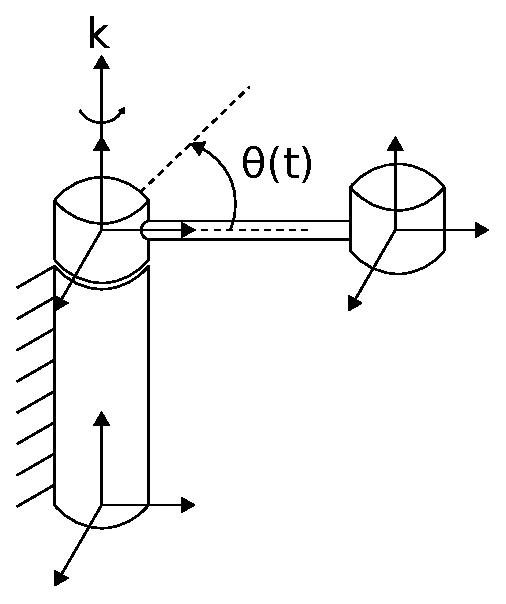
\includegraphics[width=0.5\textwidth]{figures/simple_rot.eps} 
%                 % \caption{\footnotesize Rotational motion of a one DoF manipulator.}
%             \end{figure}
%         \end{column}
%     \end{columns}

%     \begin{itemize}
%         \item In introductory dynamics courses, the computation of the linear
%         velocity $v$ is often the goal.
%         \item In our applications, we are interested in describing the motion of 
%         a moving frame:
%         \begin{itemize}
%             \footnotesize{
%             \item motion of the origin of the frame through space,
%             \item motion of the frame's axes.
%             }
%         \end{itemize}
%         \item For our purposes, the angular velocity will hold equal status with 
%         linear velocity.
%     \end{itemize}
% \end{frame}


% \begin{frame}
%     \frametitle{Angular Velocity: The Fixed Axis Case}
   

%     \begin{itemize}
%         \item The angular velocity is a property of the body-fixed coordinate
%         frame.
%         \item Angular velocity is \textit{not} a property of individual points.
%         \item Individual points may experience a \textbf{linear velocity} that 
%         is induced by an angular velocity, but it makes no sense to speak of a 
%         point itself rotating.
%         \item Thus, in equation~\eqref{eq:lin_vel_fixed}, $v$ corresponds to the 
%         linear velocity of a point, while $\omega$ corresponds to the angular 
%         velocity associated with a rotating coordinate frame.
%     \end{itemize}
% \end{frame}


% \begin{frame}
%     \frametitle{Angular Velocity: The Fixed Axis Case}

%     \begin{itemize}
%         \item In the fixed axis case, the problem of specifying angular 
%         displacements is really a planar problem
%         \begin{itemize}
%             \footnotesize{
%             \item each point traces out a circle,
%             \item every circle lies in a plane.
%             }
%         \end{itemize}
%         \item It is tempting to use $\dot{\theta}$ to represent the angular 
%         velocity.
%         \item However, this choice, does not generalize to the three-dimensional 
%         case.
%         \item We will develop a more general representation for angular velocities.
%         \item This will be analogous to our development of rotation matrices.
%         \item The key tool in this development is the skew-symmetric matrix.
%     \end{itemize}
% \end{frame}


\endgroup
\section{Lyapunov Stability Analysis on Euclidean Spaces}

\begin{frame}[standout, plain, noframenumbering]
    Lyapunov Stability Analysis on Euclidean Spaces

    % \medskip

    % \footnotesize
    % Sam Greydanus \quad Misko Dzamba \quad Jason Yosinski
\end{frame}

\begingroup
\small

\begin{frame}
    \frametitle{Autonomous Systems}

    Consider the autonomous system 
    \begin{equation}
        \dot{x} = f(x)
        \label{eq:autonomous}
    \end{equation}
    where $f: D \subseteq \mathbb{R}^n \rightarrow \mathbb{R}^n$ is a locally
    Lipschitz map, with an equilibrium point at $x = 0$.

    \begin{definition}
        The equilibrium point $x=0$ of the system~\eqref{eq:autonomous} is
        \begin{itemize}
            \item \textit{stable} if, $\forall \varepsilon > 0$, $\exists \delta
            = \delta(\varepsilon) > 0$ such that 
            \[
                \norm{x(0)}{} < \delta \; \Rightarrow \; \norm{x(t)}{} < 
                \epsilon, \; \; \forall t \geq 0.
            \]
            \item \textit{unstable} if it is not stable.
            \item \textit{asymptotically stable} if it is stable and $\delta$
            can be chosen s.t.
            \[ \norm{x(0)}{} < \delta \; \Rightarrow \; \lim_{t \to \infty} x(t)
            = 0. \]
        \end{itemize}
    \end{definition}
\end{frame}


\begin{frame}
    \frametitle{Example -- Pendulum}

    The pendulum equation
    \begin{align*}
        \dot{x}_1 &= x_2 \\
        \dot{x}_2 &= -a \sin{x_1} - b x_2
    \end{align*}
    has two equilibrium points at ($x_1 = 0$, $x_2 = 0$) and ($x_1 = \pi$, $x_2
    = 0$).
    %
    \begin{itemize}
        \item If $b=0$, trajectories in the nbhd. of the first equilibrium are 
        closed orbits.
        \item By starting sufficiently close to the eq. point, trajectories are 
        guaranteed to stay within any specified ball.
        \item The point is not asymptotically stable since trajectories don't
        tend to the eq. point.
        \item If $b > 0$, the origin becomes asymptotically stable.
        \item The second eq. point is a saddle point: the $\varepsilon-\delta$
        requirement cannot be satisfied (for every $\varepsilon > 0$ there
        exists a trajectory that will leave the ball $B_\varepsilon$ even if
        $x(0)$ is arbitrarily close to $(\pi, 0)$).
    \end{itemize}
\end{frame}


\begin{frame}
    \frametitle{Lyapunov Stability Theorem}

    \begin{theorem}
        Let $x=0 \in D$ be an equilibrium point for~\eqref{eq:autonomous}. Let
        $V: D \rightarrow \mathbb{R}$ be a continuously differentiable function
        such that
        \begin{align*}
            V(0) = 0 \; &\text{ and } \; V(x) > 0 \text{ in } D - \{0\}, \\
            &\dot{V}(x) \leq 0 \text{ in } D.
        \end{align*}
        Then, $x=0$ is stable. Moreover, if
        \[ \dot{V}(x) < 0 \text{ in } D - \{0\} \] then $x=0$ is asymptotically
        stable.
    \end{theorem}
\end{frame}


\begin{frame}
    \frametitle{Lyapunov Stability Theorem}

    \begin{proof}[Proof of stability]
        Given $\varepsilon > 0$, choose $0 < r \leq \varepsilon$ such that $B_r
        \subseteq D$. Let $\alpha = \min_{\norm{x}{}=r} V(x)$. Then, $\alpha >
        0$. Take $0 < \beta < \alpha$ and consider $\mc{M}_\beta = V^{-1}((0,
        \beta])$.

        \underline{Claim}: $\mc{M}_\beta \subseteq \accentset{\circ}{B}_r$.
        Argue ad absurdum. Suppose $\mc{M}_\beta \cap \accentset{\circ}{B}_r
        \subsetneq \mc{M}_\beta$. Then $\exists p \in \mc{M}_\beta \cap \partial B_r$.
        Note, $V(p) \geq \alpha > \beta$, but $V(\mc{M}_\beta) \subseteq
        [0,\beta]$. \hfill $\blacklozenge$

        The set $\mc{M}_\beta$ is invariant since \[ \dot{V}(x(t)) \leq 0 \;
        \Rightarrow \; V(x(t)) \leq V(x(0)) \leq \beta, \; \forall t \geq 0. \]

        Because $\mc{M}_\beta$ is compact (closed and bounded), we conclude that
        the ODE~\eqref{eq:autonomous} has a unique solution $\forall t \geq 0$
        whenever $x(0) \in \mc{M}_\beta$. Since $V$ is continuous and $V(0) =
        0$, $\exists \delta > 0$ such that \[ \norm{x}{} \leq \delta \;
        \Rightarrow \; V(x) < \beta. \]
    \end{proof}
\end{frame}

\begin{frame}
    \frametitle{Lyapunov Stability Theorem}

    \begin{proof}[Proof of stability (cont'd)]
        Then, \[ B_\delta \subseteq \mc{M}_\beta \subseteq B_r \] and 
        \[ x(0) \in B_\delta \; \Rightarrow \; x(0) \in \mc{M}_\beta \;
        \Rightarrow \; x(t) \in \mc{M}_\beta \; \Rightarrow \; x(t) \in B_r, \]
        proving stability. \hfill \qed
    \end{proof}

    \begin{figure}[bth]
        \centering
        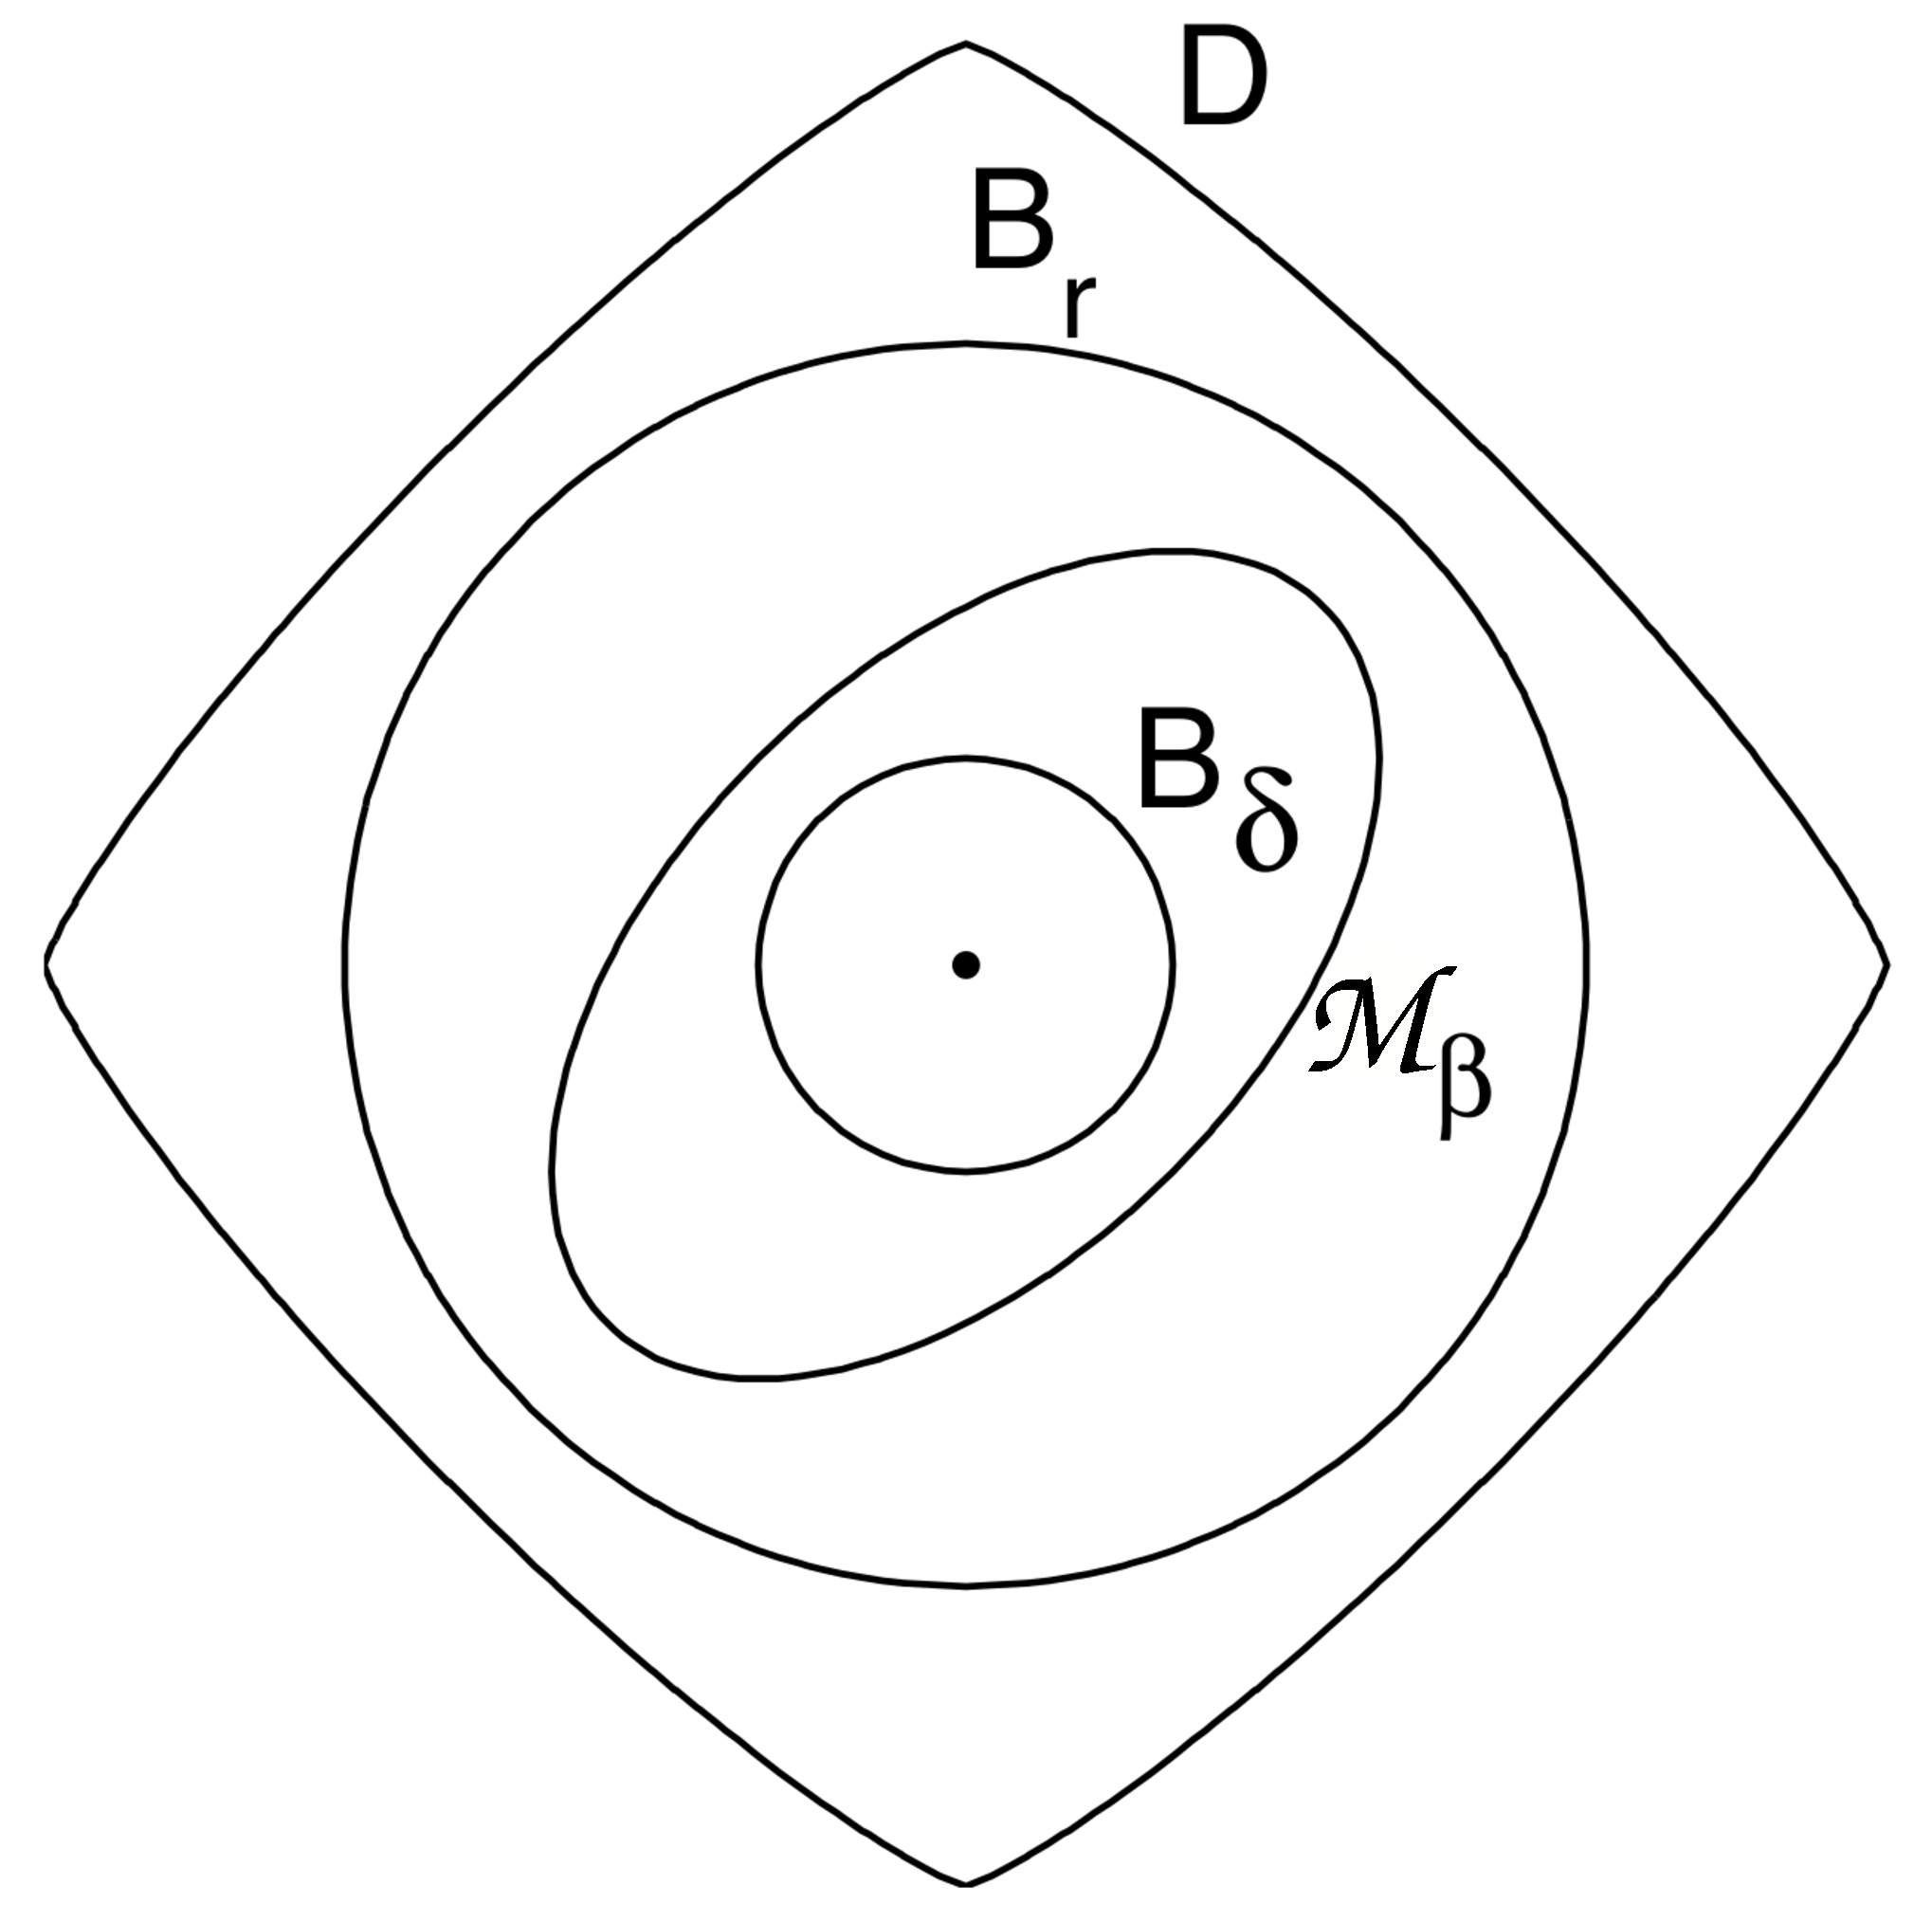
\includegraphics[width=0.35\textwidth]{figures/lyap_geometry.eps} 
        \caption{\footnotesize Geometric representation of Lyapunov stability.}
    \end{figure}
\end{frame}

\begin{frame}
    \frametitle{Lyapunov Stability Theorem}

    \begin{proof}[Proof of asymptotic stability]
        Now assume $\dot{V}(x) < 0$ in $D - \{0\}$. We want to show that $x(t)
        \xrightarrow{t \to \infty} 0$; i.e., $\forall a > 0$, $\exists T > 0$, 
        s.t. $\norm{x(t)}{} < a, \forall t > T$.

        We know that $\forall a > 0$, we can choose $b > 0$ s.t. $\mc{M}_b
        \subseteq B_a$. Therefore, it is sufficient to show that $V(x(t))
        \xrightarrow{t \to \infty} 0$. Since $V$ is monotonically decreasing and
        bounded from below by zero, \[ V(x(t)) \xrightarrow{t \to \infty} c \geq
        0. \]

        \underline{Claim}: $c = 0$. Argue ad absurdum. Suppose $c > 0$. By
        continuity of $V$, $\exists d > 0$ s.t. $B_d \subseteq \mc{M}_c$. The
        limit $V(x(t)) \rightarrow c > 0$ implies that $x(t) \notin B_d, \forall
        t \geq 0$. Define $\max_{d \leq \norm{x}{} \leq r} \dot{V}(x) =: -\gamma
        < 0$. It follows that 
        \[
        V(x(t)) = V(x(0)) + \int_0^t \dot{V}(x(\tau)) \dd \tau \leq V(x(0)) - \gamma t.
        \]
        The RHS will eventually become negative: contradiction ($c > 0$). \hfill 
        \qed
    \end{proof}
\end{frame}


\begin{frame}
    \frametitle{Lyapunov Stability: Intuition}
    \begin{figure}[bth]
        \centering
        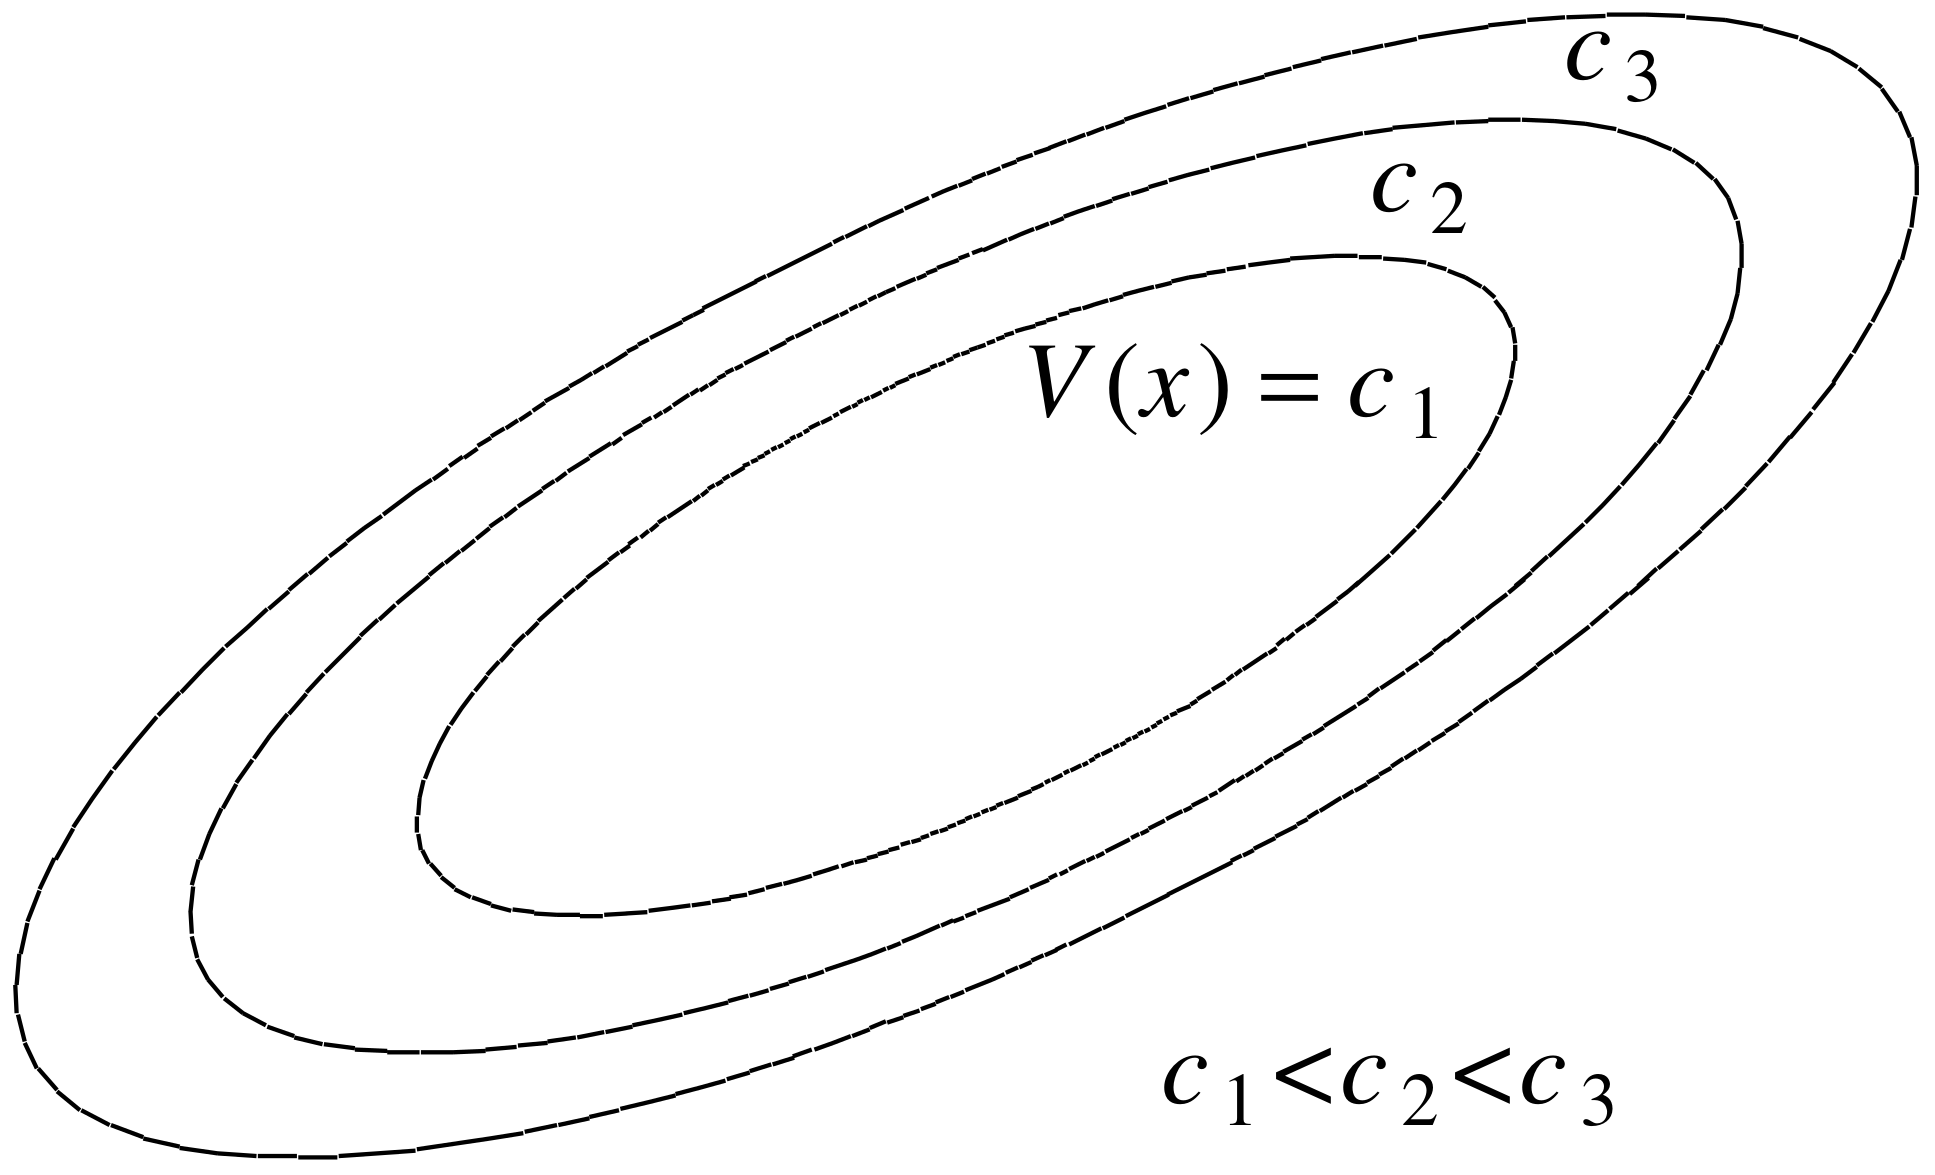
\includegraphics[width=0.35\textwidth]{figures/lyap_level_sets.png} 
        % \caption{\footnotesize Geometric representation of Lyapunov stability.}
    \end{figure}

    \begin{itemize}
        \item A continuously differentiable function $V$, satisfying the
        theorem's conditions is called a \textsc{Lyapunov function}.
        \item When $\dot{V} < 0$, the trajectory moves from level set
        $\mc{M}_{c_3} = V^{-1}(c_3)$ to an inner level set $\mc_{M}_{c_2} =
        V^{-1}(c_2)$ with a smaller $c$.
        \item $V^{-1}(c) \xrightarrow{c \downarrow 0} 0$. Hence the trajectory
        approaches the origin.
        \item If we only knew that $\dot{V} \leq 0$, we cannot be sure that the
        trajectory $x(t) \xrightarrow{t \to \infty} 0$,\footnotemark but we can
        conclude that the origin is stable.
    \end{itemize}

    \footnotetext{See, however, Krasovskii-LaSalle's theorem.}
\end{frame}


\begin{frame}
    \frametitle{Example: Undamped pendulum}

    \begin{columns}
        \begin{column}{0.5\textwidth}
            \begin{align*}
                \dot{x}_1 &= x_2, \\
                \dot{x}_2 &= -a \sin{x_1}.
            \end{align*}
        \end{column}
        \begin{column}{0.5\textwidth}
            \underline{Lyapunov function candidate}\\[0.75ex]
            $ V(x) = a(1 - \cos{x_1}) + \frac{1}{2}x_2^2. $
        \end{column}
    \end{columns}
    \begin{block}{Analysis}
        Clearly, $V(0) = 0$ and $V(x) > 0$ if $x \neq (2 k \pi, 0)$. Compute the 
        Lie derivative of $V$ along $f$:
        \[ \dot{V}(x) = \mc{L}_fV(x) = a x_2 \sin{x_1} - a x_2 \sin{x_1} = 0. \]
        Thus, the origin is stable. Since $\dot{V}(x) \equiv 0$, we conclude
        that the origin is not asymptotically stable as solutions starting on
        the level set $\mc{M}_c$ remain in that set.
    \end{block}
\end{frame}


\begin{frame}
    \frametitle{Example: Damped pendulum}

    \begin{columns}
        \begin{column}{0.5\textwidth}
            \begin{align*}
                \dot{x}_1 &= x_2, \\
                \dot{x}_2 &= -a \sin{x_1} - bx_2.
            \end{align*}
        \end{column}
        \begin{column}{0.5\textwidth}
            \begin{center}
                \underline{Lyapunov function candidate}
            \end{center}
            \vspace{-5mm}
            \begin{align*}
                V(x) &= a(1 - \cos{x_1}) + \frac{1}{2}x^\top P x, \\
                P &= P^\top > 0.
            \end{align*}
        \end{column}
    \end{columns}
    The Lie derivative $\dot{V}(x)$ is given by 
    \begin{equation*}
        \dot{V}(x) = a(1-p_{22})x_2 \sin{x_1} - ap_{12}x_1 \sin{x_1} + (p_{11} - p_{12}b)x_1x_2 + (p_{12}-p_{22}b)x_2^2.
    \end{equation*}

    \begin{itemize}
        \item Take $p_{22} = 1$ and $p_{11} = bp_{12}$.
        \item We must choose $0 < p_{12} < b$ for $V$ to be positive definite. 
        \item Choose $p_{12} = \frac{b}{2}$.
    \end{itemize}

     \begin{equation*}
        \dot{V}(x) = -\frac{1}{2}a b x_1 \sin{x_1} - \frac{1}{2}bx_2^2.
     \end{equation*}

     This is negative definite for any $0 < \abs{x_1} < \pi$.
\end{frame}


\begin{frame}
    \frametitle{Example: Rotational Motion of a Rigid Body in $3$D-space}

    With respect to a coordinate system frame, which is rigidly attached to the
    body and whose axes are chosen to be the principal axes of the body, define:
    \begin{itemize}
        \item $\omega$: angular velocity of the body,
        \item $I \in \mathbb{S}_{++}^3$: inertia matrix of the body.
    \end{itemize}
    In the absence of external torques, the motion is described by
    \begin{columns}
        \begin{column}{0.5\textwidth}
            \[ I \dot{\omega} + \omega \times I \omega = 0. \]
        \end{column}
        \begin{column}{0.5\textwidth}
            \begin{align*}
                I_x \dot{\omega}_x &= - (I_z - I_y) \omega_y \omega_z, \\
                I_y \dot{\omega}_y &= - (I_x - I_z) \omega_x \omega_z, \\
                I_z \dot{\omega}_z &= - (I_y - I_x) \omega_x \omega_y.
            \end{align*}
        \end{column}
    \end{columns}
\end{frame}


\begin{frame}
    \frametitle{Example: Rotational Motion of a Rigid Body in $3$D-space}

    Suppose w.l.o.g., that $I_x \geq I_y \geq I_z > 0$. For notational
    simplicity, define
    \begin{columns}
        \begin{column}{0.5\textwidth}
            \begin{align*}
                \omega_x &\mapsto x \\
                \omega_y &\mapsto y \\
                \omega_z &\mapsto z
            \end{align*}
        \end{column}
        \begin{column}{0.5\textwidth}
            \begin{align*}
                a &= \frac{I_y - I_z}{I_x}, \\
                b &= \frac{I_x - I_z}{I_y}, \\
                c &= \frac{I_x - I_y}{I_z}.
            \end{align*}
        \end{column}
    \end{columns}
    Note that $a, b, c, \geq 0$. The equations of motion assumes the form
    \[ \dot{x} = ayz, \;\; \dot{y} = -bxz, \;\; \dot{z} = cxy. \]

    From here on out, assume that the principal axes are unique; this is
    equivalent to assuming that $I_x > I_y > I_z$, or that $a, b, c > 0$.
\end{frame}

\begin{frame}
    \frametitle{Example: Rotational Motion of a Rigid Body in $3$D-space}

    The set of equilibria is \[ \left( \mathbb{R} \times \{0\} \times \{0\}
    \right) \cup \left( \{0\} \times \mathbb{R} \times \{0\} \right) \cup
    \left( \{0\} \times \{0\} \times \mathbb{R} \right). \] \vspace{-4mm}
    \begin{block}{Remark}
        Physically this corresponds to rotation around one of the principal axes
        at a constant angular velocity. Note that none of the equilibria is
        isolated.
    \end{block}
    \vspace{-2mm}
    Consider first, the equilibrium at the origin and try \[ V(x,y,z) = px^2 +
    qy^2 + rz^2, \] where $p,q,r > 0$. Then $V$ is a lpdf. Computing $\dot{V}$:
    \[ \dot{V} = 2(px\dot{x} + qy\dot{y} + rz\dot{z}) = 2xyz(ap - bq + cr). \]
    Clearly, it is possible to choose $p,q,r > 0$ such that \[ ap - bq + cr = 0.
    \] For such a choice, $\dot{V} \equiv 0$ and the origin is \textsc{stable}.
\end{frame}


\begin{frame}
    \frametitle{Example: Rotational Motion of a Rigid Body in $3$D-space}

    Next, consider the equilibrium of the form $(x_0, 0, 0)$ where $x_0 \neq 0$.

    Consider the Lyapunov function candidate $W$, such that $W(x_0, 0, 0) = 0$,
    and $W(x,y,z) > 0, \; \forall (x,y,z) \neq (x_0, 0, 0)$ and sufficiently
    near $(x_0, 0, 0)$: \[ W(x,y,z) = cy^2 + bz^2 + \left[ 2acy^2 + abz^2 +
    bc(x^2 - x_0^2) \right]^2 \]

    $W$ is an lpdf w.r.t. the equilibrium $(x_0, 0, 0)$ and routine computations 
    show that $\dot{W} \equiv 0$. Hence $(x_0, 0, 0)$ is a stable equilibrium.

    \begin{block}{Discussion}
        \begin{itemize}
            \item We could also translate the coordinates such that $(x_0, 0,
            0)$ becomes the origin of the new coordinate system and apply the
            Lyapunov stability theorem directly.
            \item Is $(0, 0, z_0)$, $z_0 \neq 0$ stable?
            \item Is $(0, y_0, 0)$, $y_0 \neq 0$ (w.l.o.g., assume $y_0 > 0$)
            stable?
        \end{itemize}
    \end{block}
\end{frame}


\begin{frame}
    \frametitle{Region of Attraction}

    \begin{definition}[Region of Attraction]
        The \textsc{region of attraction} is defined as the set of all points
        $x$ such that $\phi(t; x)$ is defined for all $t \geq 0$ and $\lim_{t
        \to \infty} \phi(t; x) = 0$.
    \end{definition}
    \begin{itemize}
        \item Finding the exact RoA is usually difficult.
        \item Lyapunov fcns. can be used to estimate (inner approx.) the RoA.
        \item From the proof of the Lyapunov stability theorem, if there is a
        Lyapunov fcn. that satisfies asymptotic stability and if $\mc{M}_c$ is
        bounded and contained in $D$, then $\mc{M}_c$ is (positively) invariant.
        \item The estimate $\mc{M}_c$ of the RoA may be conservative (inner
        approximation).
        \item \textsc{Question}: Under what conditions is the RoA the whole space?
        \begin{itemize}
            \item If so, the origin is said to be \textit{globally asymptotically stable}.
            \item The conditions of the Lyapunov theorem must clearly hold for
            $D = \mathbb{R}^n$. But is this sufficient?
        \end{itemize}
    \end{itemize}
\end{frame}


\begin{frame}
    \frametitle{Region of Attraction}
    \only<1>{
    \begin{figure}[bth]
        \centering
        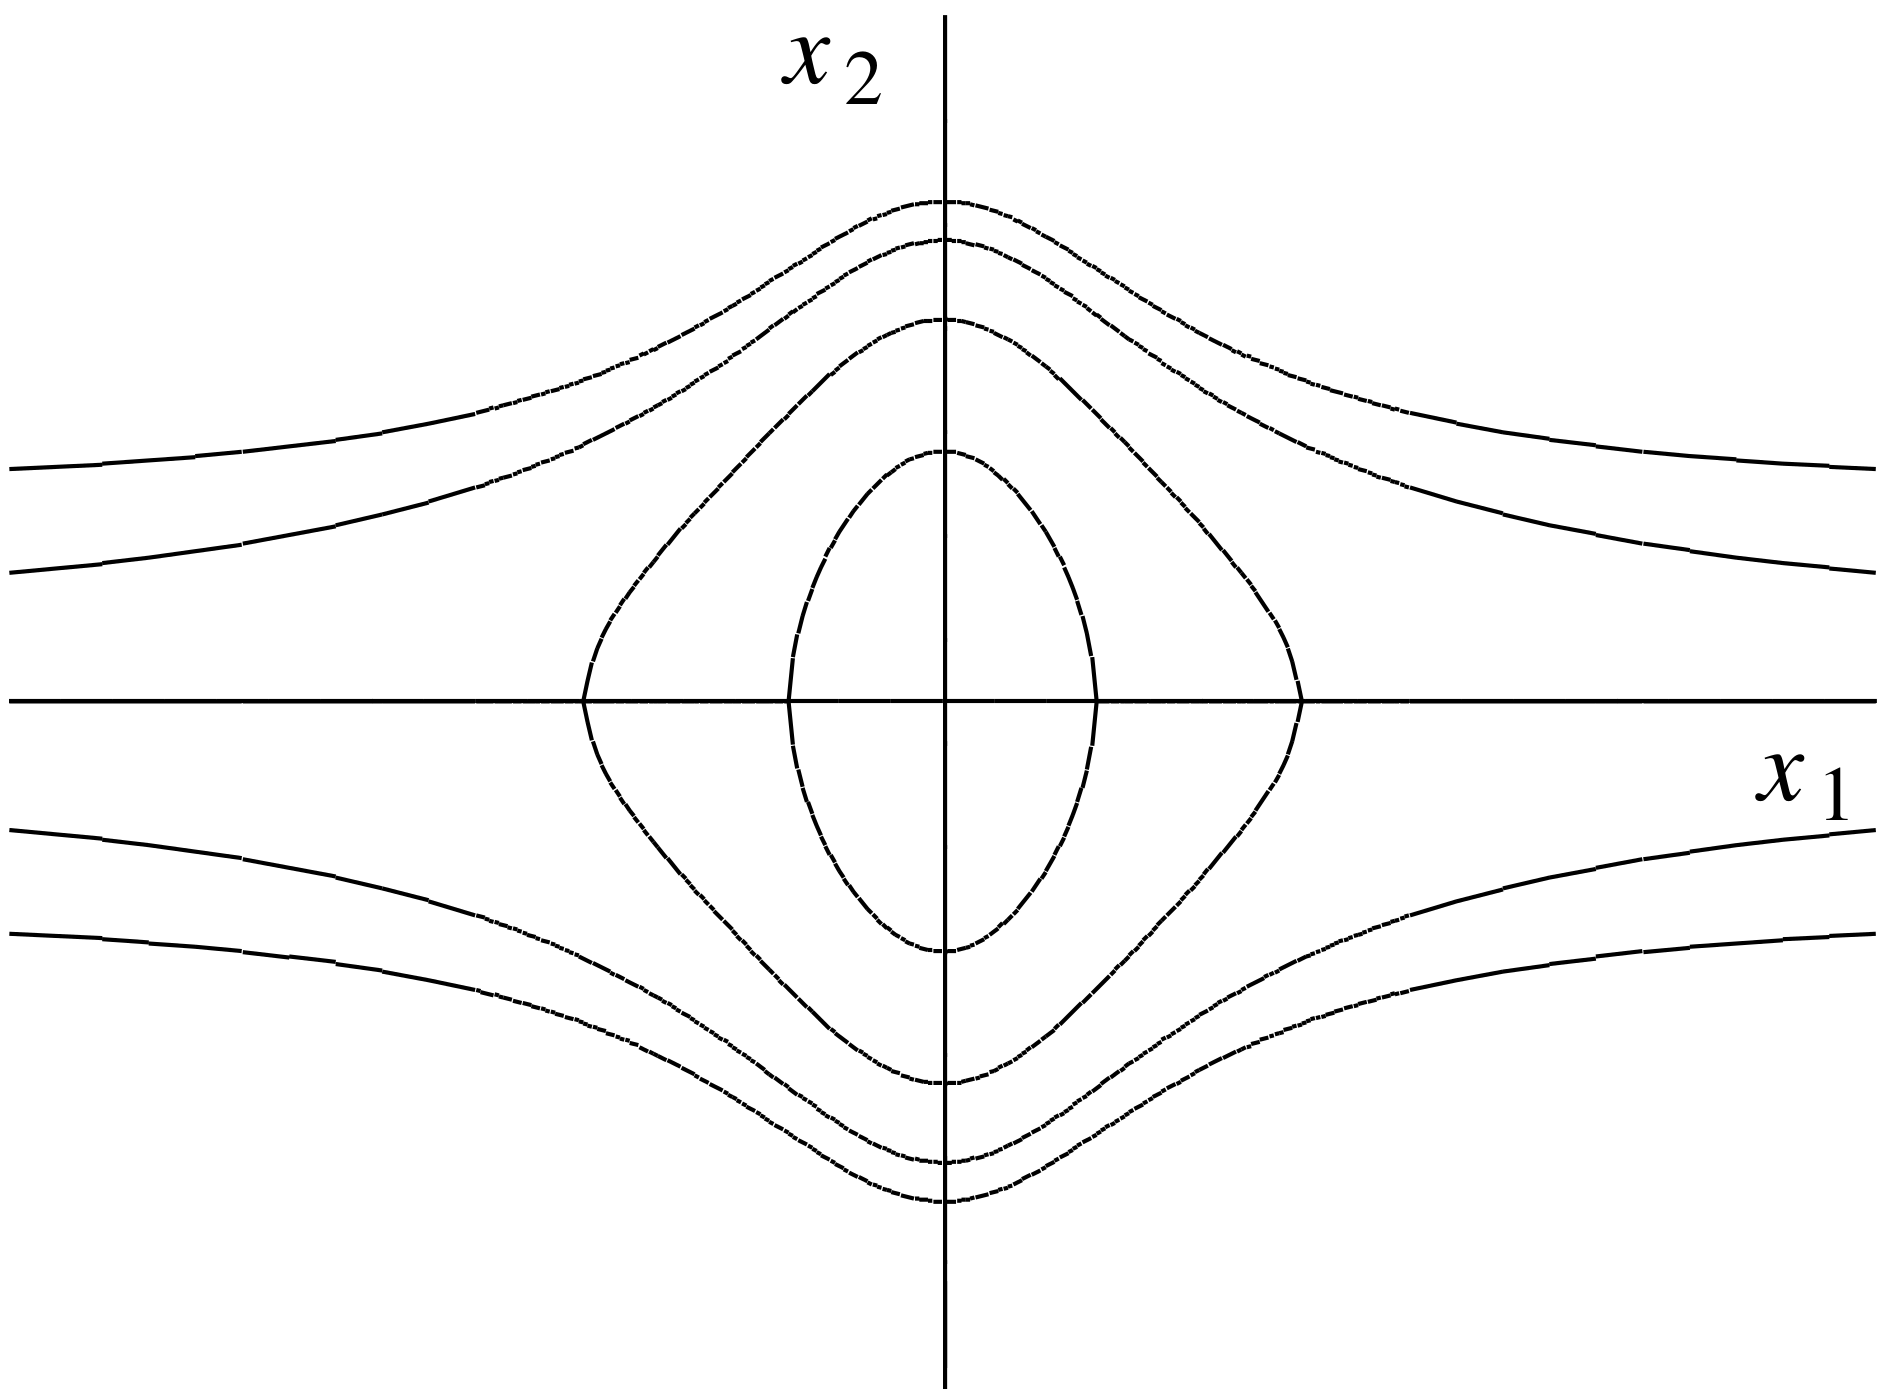
\includegraphics[width=0.35\textwidth]{figures/lyap_surfaces.png} 
        \caption{\footnotesize Level sets of $V(x) = \frac{x_1^2}{1 + x_1^2} + x_2^2$.}
    \end{figure}
    \vspace{-4mm}
    }
    For $\mc{M}_c$ to be bounded ($\mc{M}_c \subseteq \accentset{\circ}{B}_r$,
    for some $r \geq 0$), $c < \inf_{\norm{x}{} \geq r}V(x)$. If \[ l = \lim_{r
    \to \infty} \inf_{\norm{x}{} \geq r} V(x) < \infty \] then $\mc{M}_c$ will be bounded only if $c < l$.
    Consider (see figure) \[ V(x) =
    \frac{x_1^2}{1 + x_1^2} + x_2^2. \] In this example, 
    \[ l = \lim_{r \to \infty} \min_{\norm{x}{}=r} V(x) = 1. \] 

    \onslide<2->{
    An extra
    condition that ensures that $\mc{M}_c$ is bounded for all $c > 0$ is \[ V(x)
    \to \infty \; \text{ as } \; \norm{x}{} \to \infty. \]
    }
    \vspace{-5mm}
    \begin{block}{Homework}
        Show that a continuously differentiable map $V: \mathbb{R}^n \rightarrow
        \mathbb{R}$ is radially unbounded if and only if it is proper (inverse
        images of compact sets under $V$ are compact).
    \end{block}
\end{frame}

\begin{frame}
    \frametitle{Region of Attraction}

    \begin{theorem}[Global Asymptotic Stability]
        Let $V: \mathbb{R}^n \rightarrow \mathbb{R}$ be a continuously
        differentiable function and the conditions of the Lyapunov stability
        theorem hold (\textit{asymptotic}). If, in addition, \[ \norm{x}{} \to
        \infty \; \Rightarrow \; V(x) \to \infty \] then $x=0$ is
        \textit{globally asymptotically stable}.
    \end{theorem}
    
    \begin{rem}
        For $x=0$ to be GAS, it must be the unique equilibrium point of the
        system (why?).
    \end{rem}
\end{frame}


\begin{frame}
    \frametitle{Chetaev's Instability Theorem}

    \begin{theorem}
        Let $V: D \rightarrow \mathbb{R}$ be a continuously differentiable
        function such that $V(0) = 0$ and $V(x_0) > 0$ for some $x_0$ with
        arbitrarily small $\norm{x_0}{}$. Let\\[0.5ex] \hspace{35mm} $U := \{ x
        \in B_r: V(x) > 0\}$\\[0.5ex] and suppose that $\dot{V}(U) > 0$. Then,
        $x=0$ is unstable.
    \end{theorem}

    \begin{proof}
        $x_0 \in \accentset{\circ}{U}$ and $V(x_0) = a > 0$. The trajectory
        $x(t)$ starting at $x(0) = x_0$ must leave $U$. Indeed, as long as $x(t)
        \in U$, $V(x(t)) \geq a$, since $\dot{V}(U) > 0$. Let $\min 
        \{\dot{V}(x): x \in U \text{ and } V(x) \geq a \} := \gamma > 0$.  Then, 
        \[ V(x(t)) = V(x_0) + \int_0^t \dot{V}(x(s)) \dd s \geq a + \int_0^t
        \gamma \dd s = a + \gamma t. \] Hence, $x(t)$ will leave $U$ because
        $V(x)$ is bounded on $U$. Now, $x(t)$ cannot leave $U$ through $V(x) =
        0$ since $V(x(t)) \geq a$. Hence it must leave $U$ through the sphere
        $\mathbb{S}_r$. Note: $\norm{x_0}{}$ was arbitrarily small. \hfill \qed
    \end{proof}
\end{frame}


\begin{frame}
    \frametitle{Example: Rotational Motion of a Rigid Body}

    Consider an equilibrium of the form $(0, y_0, 0)$, $y_0 > 0$ and translate
    the coordinates so that the equilibrium under study becomes the origin.
    Setting $y_s = y - y_0$, the equations of motion are
    \[ \dot{x} = ay_sz + ay_0z, \;\; \dot{y}_s = -bxz, \;\; \dot{z} = cxy_s +
    cxy_0. \] Now, apply Chetaev's theorem with 
    \begin{align*}
        V(x,y,z) &= xz, \\
        B_r &= \{ (x,y_s,z): x^2 + y_s^2 + z^2 < r^2 \}, \\
        U &= \{ (x,y_s,z) \in B_{\frac{r}{2}}: x > 0 \text{ and } z > 0 \}.
    \end{align*}
    Then $U$ is open and \[ \dot{V} = x\dot{z} + \dot{x}z = 2(y_s + y_0)(cx^2 +
    az^2). \] If $(x,y_s,z) \in U$, then $y_s + y_0 > 0$, so Chetaev's theorem 
    yields that the origin (in the new coordinate system) is \textsc{unstable}.
\end{frame}

\endgroup
\section{The Invariance Principle}

\begin{frame}[standout, plain, noframenumbering]
    The Invariance Principle

    % \medskip

    % \footnotesize
    % Sam Greydanus \quad Misko Dzamba \quad Jason Yosinski
\end{frame}

\begingroup
\small


\begin{frame}
    \frametitle{Intuition}

    
\end{frame}


\endgroup
\section{Stability of Linear Systems}

\begin{frame}[standout, plain, noframenumbering]
    Stability of Linear Systems

    % \medskip

    % \footnotesize
    % Sam Greydanus \quad Misko Dzamba \quad Jason Yosinski
\end{frame}

\begingroup
\small



\begin{frame}
    \frametitle{Autonomous Linear Systems}

    We restrict our attention to linear \textit{autonomous} systems of the form 
    \begin{equation}
        \dot{x}(t) = A x(t).
        \label{eq:lin_system}
    \end{equation}

    \begin{theorem}
        The equilibrium $0$ of~\eqref{eq:lin_system} is (globally) exponentially
        stable if and only if all eigenvalues of $A$ have negative real parts.
        The equilibrium is stable if and only if all eigenvalues of $A$ have
        nonpositive real parts, and in addition, every eigenvalue of $A$ having
        a zero real part is a simple zero of the minimal polynomial of $A$.
    \end{theorem}
\end{frame}

\begin{frame}
    \frametitle{Lyapunov Function}

    Given the system~\eqref{eq:lin_system}, we choose a Lyapunov function
    candidate: \[ V(x) = x^\top P x \implies \dot{V} = \dot{x}^\top P x + x^\top
    P \dot{x} = - x^\top Q x, \] where $P = P^\top$ and 
    \begin{equation}
        A^\top P + PA = -Q.
        \label{eq:lyap_matrix}
    \end{equation}
    Equation~\eqref{eq:lyap_matrix} is commonly known as the \textbf{Lyapunov
    Matrix Equation}.
    \begin{rem}[Stability]
        If a pair of matrices $(P, Q)$ satisfying~\eqref{eq:lyap_matrix} can be
        found such that both $P$ and $Q$ are positive definite, then both $V$
        and $-\dot{V}$ are positive definite functions and $V$ is radially
        unbounded. Hence, the equilibrium $0$ is globally exponentially stable.

        If a pair $(P, Q)$ can be found s.t. $Q > 0$ and $P$ has at least one
        nonpositive eigenvalue, then $-\dot{V} > 0$ and $V$ assumes nonpositive
        values arbitrarily close to the origin. Hence $0$ is unstable.
    \end{rem}
\end{frame}


\begin{frame}
    \frametitle{Lyapunov Matrix Equation}

    \begin{lemma}
        Let $\{\lambda_i\}_1^n$ denote the eigenvalues of $A$. Then
        equation~\eqref{eq:lyap_matrix} has a unique solution for $P$
        corresponding to each $Q \in \mathbb{R}^{n \times n}$ iff \[ \lambda_i +
        \lambda_j \neq 0, \;\; \forall i, j. \]
    \end{lemma}

    \begin{corollary}
        If for some $Q \in \mathbb{R}^{n \times n}$ does not have a unique
        solution for $P$, then the origin is not an asymptotically stable
        equilibrium.
    \end{corollary}
    \begin{proof}
        If all eigenvalues of $A$ has negative real parts, then the equation 
        above is satisfied. \hfill \qed
    \end{proof}
\end{frame}


\begin{frame}
    \frametitle{Main Result}

    \begin{theorem}
        Given a matrix $A \in \mathbb{R}^{n \times n}$, the following are
        equivalent:
        \begin{itemize}
            \item $A$ is a Hurwitz matrix (all its e.vals have negative real parts).
            \item There exists \textsc{some} $Q \in \mathbb{S}_{++}^n$ such that
            equation~\eqref{eq:lyap_matrix} has a corresponding unique solution
            for $P \in \mathbb{S}_{++}^n$.
            \item For \textsc{every} $Q \in \mathbb{S}_{++}^n$,
            equation~\eqref{eq:lyap_matrix} has a unique solution for $P \in
            \mathbb{S}_{++}^n$.
        \end{itemize}
    \end{theorem}
    \begin{proof}
        ``$(3) \implies (2)$'' Obvious. \\
        ``$(2) \implies (1)$'' Suppose $(2)$ is true for some particular matrix
        $Q$. Consider the candidate $V(x) = x^\top P x$. Then $\dot{V}(x) =
        -x^\top Q x$, and one can conclude that $0$ is asymptotically stable. 
        Hence $A$ is Hurwitz. \\
        ``$(1) \implies (3)$'' Omitted (see Section 5.4, Theorem (42) in
        Vidyasagar, ``\textit{Nonlinear Systems Analysis}'', 1993.)
    \end{proof}
\end{frame}


\endgroup
\section{Control-Lyapunov Functions}

\begin{frame}[standout, plain, noframenumbering]
    Control-Lyapunov Functions

    % \medskip

    % \footnotesize
    % Sam Greydanus \quad Misko Dzamba \quad Jason Yosinski
\end{frame}

\begingroup
\small

\begin{frame}
    \frametitle{Control-Lyapunov Functions~\footnote[1]{As discussed in
        \textit{Sontag, ``A `universal' construction of Artstein's theorem on
        nonlinear stabilization''}, 1989.}}

    Consider the control system with state $x \in \mathbb{R}^n$ and control
    $u \in \mathbb{R}^m$, $\forall t$:
    \begin{equation}
        \dot{x}(t) = f(x(t)) + u_1(t)g_1(x(t)) + \cdots + u_m(t)g_m(x(t)), \;\;\; f(0) = 0.
        \label{eq:ctrl_system}
    \end{equation}

    \begin{definition}[Control-Lyapunov Function (clf)]
        A clf is a smooth, proper, and positive definite function $ V:
        \mathbb{R}^n \rightarrow \mathbb{R} $ so that
        \[\inf_{u \in \mathbb{R}^m}\{ \mc{L}_fV(x) + u_1 \mc{L}_{g_1}V(x) +
        \cdots + u_m \mc{L}_mg_M V(x) \} < 0, \;\; \forall x \neq 0. \]
    \end{definition}

    \vspace{-3mm}
    \begin{itemize}
        \item $V$ is such that for each $x \neq 0$, one \textit{can} diminish
        its value by applying \textit{some} open-loop control.
        \item Existence of a clf implies that the system is asymp. controllable: 
    \end{itemize}
    \vspace{2mm}
\end{frame}

\begin{frame}
    \frametitle{Control-Lyapunov Functions: Single input}
    There exists a feedback law which is smooth on $\mathbb{R}_0^n :=
    \mathbb{R}^n - 0$
    \vspace{-1mm}
    \begin{equation*}
        u = k(x), \quad k(0) = 0,
        \vspace{-1mm}
    \end{equation*}
    and which globally stabilizes the system.

    Assume $V$ is a clf for the system
    \vspace{-1mm}\[ \dot{x} = f(x) + u g(x) \vspace{-1mm}. \] Denote
    \vspace{-3mm}
    \begin{align*}
        a(x) &:= \nabla V(x) \cdot f(x), \\
        b(x) &:= \nabla V(x) \cdot g(x).
        \vspace{-3mm}
    \end{align*}
    The condition that $V$ is a clf is precisely the statement that 
    \[ b(x) = 0 \implies a(x) < 0, \quad \forall x \neq 0. \] On the other hand,
    $V$ is a Lyapunov function if \vspace{-1mm}\[ \nabla V(x) \cdot \left( f(x)
    + k(x)g(x) \right) < 0, \] that is \[ a(x) + k(x) b(x) < 0, \quad \forall x
    \neq 0. \]
\end{frame}


\begin{frame}
    \frametitle{Control-Lyapunov Functions: Single input}

    In this simple case where the family $\left( a(x), b(x) \right)$,
    interpreted as a \textit{family of linear systems parametrized by $x$} the
    following works: \[ k := -\frac{1}{b}\left( a + \sqrt{a^2 +
    b^2} \right). \] Along trajectories of the closed-loop system, one has 
    \[ \frac{\dd V}{\dd t} = -\sqrt{a^2 + b^2} < 0. \] This feedback law may
    fail to be continuous, but with the slight modification \[ k :=
    -\frac{1}{b}\left( a + \sqrt{a^2+b^4} \right), \] then it does become
    continuous.
\end{frame}


\begin{frame}
    \frametitle{Control-Lyapunov Functions: Multi input}

    Now, consider the system back in equation~\eqref{eq:ctrl_system}. 
    
    \begin{itemize}
        \item A sufficient conditions for a given $k$ to be smooth feedback
        stabilizer is that there exist a Lyapunov function $V$ so that \[ \nabla
        V(x) \cdot \left[ f(x) + k_1(x)g_1(x) + \cdots + k_m(x)g_m(x) \right] <
        0, \;\; \forall x \neq 0. \] 
        \item Such a Lyapunov function is automatically a clf.
        \item If $k$ happens to be continous at the origin, then the following
        property (\texttt{small control property}) holds (with $u := k(x)$) \\
        \textit{
            For each $\varepsilon > 0$, there is $\delta > 0$ s.t., if $x \neq 0$ 
            satisfies $\norm{x}{} < \delta$, then there is some 
            $u$ with $\norm{u}{} < \varepsilon$ s.t.
            \[\nabla V(x) \cdot \left[ f(x) + u_1g_1(x) + \cdots + u_mg_m(x) 
            \right] < 0. \]
        }
    \end{itemize}
\end{frame}


\begin{frame}
    \frametitle{Control-Lyapunov Functions: Multi input}

    \begin{theorem}
        If $\exists$ a smooth clf $V$ then $\exists$ a smooth feedback
        stabilizer $k$. If $V$ satisfies the small control property, then $k$ 
        can be chosen to be also continuous at $0$.
    \end{theorem}

    \begin{proof}[Proof. (Sketch)]
        The proof involves constructing a fixed function $\phi$ of two
        variables, and then designing a feedback law in closed-form, from the
        evaluation of this function at a point determined by $\nabla V(x) \cdot
        f(x)$ and the $\nabla V(x) \cdot g_i(x)$'s.

        Define the following function (and then show that it is analytic.)
        \[ \phi(a, 0) := 0, \quad \forall a < 0 \] and \[ \phi(a,b) :=
        \frac{1}{b}\left( a^2 + bq(b) \right), \quad q(0) = 0 \; \text{ and } \;
        bq(b) > 0. \]
        For example, we can choose $q(b) = b$ or $q(b) = b^3$, etc.
    \end{proof}
\end{frame}

\begin{frame}
    \frametitle{Control-Lyapunov Functions: Multi input}

    \begin{proof}[Proof. (Cont'd)]
        Assume that $V$ is a clf and let 
        \begin{align*}
            a(x) &:= \nabla V(x) \cdot f(x), \\
            b_i(x) &:= \nabla V(x) \cdot g_i(x), \;\; i=1,\ldots,m.
        \end{align*}
        Further, let
        \begin{align*}
            B(x) &:= (b_1(x), \ldots, b_m(x)), \\
            \beta(x) &:= \norm{B(x)}{}^2 = \sum_{i=1}^m b_i^2(x).
        \end{align*}
        The condition that $V$ is a clf is equivalent to $\beta(x) = 0 \implies
        a(x) < 0$. Now, define the smooth feedback law $k = (k_1, \ldots, k_m)$: \[
        k_i(x) := -b_i(x)\phi(a(x), \beta(x)), \quad x \neq 0, \] and $k(0) :=
        0$.
    \end{proof}
\end{frame}

\begin{frame}
    \frametitle{Control-Lyapunov Functions: Multi input}

    \begin{proof}[Proof. (Cont'd)]
        At a nonzero $x$ we have that 
        \begin{align*}
            \nabla V(x) \cdot \left[ f(x) + \sum_{i=1}^m k_i(x)g_i(x) \right]
            &= a(x) - \phi\left( a(x), \beta(x) \right)\beta(x) \\
            &= -\sqrt{a(x)^2 + \beta(x)q\left( \beta(x) \right)} < 0.
        \end{align*}
        so the original $V$ decreases along trajectories of the closed-loop
        system.

        We have still yet to show that $V$ satisfies the small control property.
        The audience is invited to see the paper for the detailed proof of this.
        \hfill \qed
    \end{proof}
\end{frame}


\endgroup
\section{Morse-Lyapunov Functions}

\begin{frame}[standout, plain, noframenumbering]
    Morse-Lyapunov Functions

    % \medskip

    % \footnotesize
    % Sam Greydanus \quad Misko Dzamba \quad Jason Yosinski
\end{frame}

\begingroup
\small

\begin{frame}
    \frametitle{Isolated Critical Points}

    \begin{lemma}
        Suppose that $x_e$ is an equilibrium points of the dynamical system $(M,
        \varphi)$. If $V: \mc{M} \rightarrow \mathbb{R}$ is a differentiable
        Lyapunov function then $x_e$ is the only critical point of $V$.
    \end{lemma}

    \begin{proof}
        Suppose $V$ has another critical point, $x_c$, in the domain of
        attraction. By the definition of a Lyapunov function, we must have
        $\mc{L}_fV(x_c) = 0$. This contradicts the fact that if $x \neq x_e$,
        $\mc{L}_fV(x) < 0$.
    \end{proof}
\end{frame}


\begin{frame}
    \frametitle{Morse Lemma}

    \begin{theorem}[Morse Lemma]
        Let $p \in \mc{M}$ be a nondegenerate critical point of a smooth
        function $V: \mc{M} \rightarrow \mathbb{R}$. There exists a local
        coordinate system $\{x_i\}_1^n$ in a nbhd. $\mc{N} \subseteq \mc{M}$ of
        $p$ with $x_i(p) = 0$ for all $1 \leq i \leq n$ such that for $x \in
        \mc{N}$, \[ V(x) = V(p) - x_1^2 - \ldots - x_i^2 + x_{i+1}^2 + \ldots +
        x_n^2 \] where $i = \text{ind}(V,p)$.
    \end{theorem}

    \begin{corollary}
        Let $p \in \mc{M}$ be an equilibrium point of $(\mc{M}, \varphi)$ and
        $V: \mc{M} \rightarrow \mathbb{R}_{\geq 0}$ a Morse-Lyapunov function. 
        There exists a local coordinate system $\{x_i\}_1^n$ around $p$ such that 
        $V$ is locally the canonical quadratic Lyapunov function 
        \[ V(x) = \sum_{i=1}^n x_i^2 \] with $\text{ind}(V, p) = 0$.
    \end{corollary}
\end{frame}


\begin{frame}
    \frametitle{Level Sets of a Lyapunov Function}

    \begin{theorem}[Deformation Lemma]
        Let $V: \mc{M} \rightarrow \mathbb{R}$ be a smooth function and $a, b
        \in V(\mc{M})$ such that $a < b$. If $\mc{M}_{a,b}$ is compact and does
        not contain critical points of $V$ then $\mc{M}_a$ is diffeomorphic to
        $\mc{M}_b$. MOreover, $\mc{M}_a$ is a deformation retract of $\mc{M}_b$.
    \end{theorem}

    \begin{corollary}
        Let $\mc{M}$ be a smooth Riemannian manifold. If $\mc{M}$ contains a
        closed invariant asymptotically stable set, then for all $a, b \in
        V(\mc{M})$, $\mc{M}_a$ is diffeomorphic to $\mc{M}_b$ and $\mc{M}_a$ is
        a deformation retract of $\mc{M}_b$ where $V$ is a smooth Lyapunov
        function.
    \end{corollary}
\end{frame}


\endgroup
\section{Systems with Single Critical Points}

\begin{frame}[standout, plain, noframenumbering]
    Systems with Single Critical Points

    % \medskip

    % \footnotesize
    % Sam Greydanus \quad Misko Dzamba \quad Jason Yosinski
\end{frame}

\begingroup
\small

\begin{frame}
    \frametitle{Domain of Attraction -- Revisited}

    \begin{theorem}[Brown-Stallings Lemma]
        Let $\mc{M}$ be a paracompact manifold such that every compact subset is
        contained in an open set diffeomorphic to a Euclidean space. Then
        $\mc{M}$ itself is diffeomorphic to a Euclidean space.
    \end{theorem}

    \begin{corollary}
        Let $\mc{M}$ be a paracompact manifold. The domain of attraction of an
        asymptotically stable equilibrium point is diffeomorphic to a Euclidean
        space.
    \end{corollary}
\end{frame}

\begin{frame}
    \frametitle{Morse and Sontag Theorems}

    \begin{theorem}[Morse Theorem]
        Let $V: \mc{M} \rightarrow \mathbb{R}$ be a Morse function, $p$ a
        critical point such that $\text{ind}(V, p) = i$ and $c = V(p)$. If there
        exists $\varepsilon > 0$ such that $\mc{M}_{c-\varepsilon,
        c+\varepsilon}$ is compact and does not contain other critical points
        $p$, then $\mc{M}_{c-\varepsilon} \cup e_i$ is a deformation retract of
        $\mc{M}_{c+\varepsilon}$ where $e_i$ is an $i$-cell.
        % (in particular, $\mc{M}_{c+\varepsilon}$ has the homotopy type of
        % $\mc{M}_{c-\varepsilon}$ with an $i$-cell attached).
    \end{theorem}

    \begin{theorem}[Sontag Theorem]
        Let us consider the dynamical system $(\mc{M}, \varphi)$ with an
        equilibrium point $x_e \in \mc{M}$. Suppose that $x_e$ is asymptotically
        stable. Then the domain of attraction of $x_e$, given by 
        \[ \mc{A} = \left\{ x \in \mc{M}: \lim_{t \rightarrow \infty} \varphi(t,
        x) = x_e \right\}, \] is contractible.
    \end{theorem}
\end{frame}


\endgroup
\section{Systems with Multiple Critical Points}

\begin{frame}[standout, plain, noframenumbering]
    Systems with Multiple Critical Points

    % \medskip

    % \footnotesize
    % Sam Greydanus \quad Misko Dzamba \quad Jason Yosinski
\end{frame}

\begingroup
\small


\begin{frame}
    \frametitle{Morse Theorem -- (Third Version)}

    \begin{theorem}[Morse Theorem]
        If $V: \mc{M} \rightarrow \mathbb{R}$ is a Morse function such that 
        $\mc{M}_a$ is compact for each $a \in \mathbb{R}$ then $\mc{M}$ has the 
        homotopy type of a CW-complex with one $i$-cell for each critical point 
        of index $i$.
    \end{theorem}
    
    \begin{corollary}
        Suppose that the dynamical system $(\mc{M}, \varphi)$ has several
        equilibria $(x_1, \ldots, x_k)$. If there exists a Morse-Lyapunov
        function $V: \mc{M} \rightarrow \mathbb{R}_{\geq 0}$ then $\{x_1,
        \ldots, x_k\}$ is a retract of the domain of attraction.
    \end{corollary}

    \begin{prop}[Reeb Theorem]
        Suppose that $\mc{M}$ is compact without boundary. If $V: \mc{M}
        \rightarrow \mathbb{R}$ is a smooth function with only two critical
        points, then $\mc{M}$ is homeomorphic to the $n$-sphere $\mathbb{S}^n$.
    \end{prop}
\end{frame}

\begin{frame}
    \frametitle{Morse Inequalities}

    \begin{theorem}[Morse Inequalities]
        Let $m_k$ be the number of ciritcal points of a Morse function $V$ with
        index $k$. Then, we have

        \begin{align*}
            b_k &\leq m_k, \quad \forall k, \\
            \sum_{i=0}^j (-1)^{j-i}b_i &\leq \sum_{i=0}^j (-1)^{j-i}m_i \quad \forall j, \\
            \chi(\mc{M}) &= \sum_k (-1)^k b_k = \sum_k (-1)^k m_k.
        \end{align*}
    \end{theorem}

    The next corollary states a necesary condition for the existence of a
    Morse-Lyapunov function based on the Euler characteristic, which is a
    topological invariant.
\end{frame}


\begin{frame}
    \frametitle{Existence of Morse-Lyapunov Functions}

    \begin{corollary}
        Consider the dynamical system $(\mc{M}, \varphi)$ with several
        equilibria $(x_1, \ldots, x_k)$. If there exists a Morse-Lyapunov
        function $V: \mc{M} \rightarrow \mathbb{R}_{\geq 0}$ then $\chi(\mc{M})
        = k \geq b_0$.
    \end{corollary}

    \begin{proof}
        If there exists a Morse-Lyapunov function $V$, $(x_1, \ldots, x_k)$ are
        the only critical points with indices $0$. Then, by the Morse
        inequalities, $\chi(\mc{M}) = m_0 = k$ and $b_0 \leq m_0 = k$.
    \end{proof}

    \begin{rem}
        If $\chi(\mc{M}) \neq k$ then there is no Morse-Lyapunov function for
        the dynamical system.
    \end{rem}
\end{frame}

\endgroup
% \section{Singularities}

\begin{frame}[standout, plain, noframenumbering]
    Singularities

    % \medskip

    % \footnotesize
    % Sam Greydanus \quad Misko Dzamba \quad Jason Yosinski
\end{frame}

\begingroup
\small


\begin{frame}
    \frametitle{Singularities}

    \begin{itemize}
        \item The $6 \times n$ Jacobian $J(q)$ defines a mapping \[ \xi =
        J(q)\dot{q} \] between the vector $\dot{q}$ of joint velocities and the
        vector $\xi = (v, \omega)$ of end effector velocities. In other words,
        \[ \xi = J_1 \dot{q}_1 + J_2 \dot{q}_2 + \cdots + J_n \dot{q}_n. \]
        \item Since $\xi \in \mathbb{R}^6$, it is necessary that $J$ have six 
        linearly independent columns for the end effector to be able to achieve 
        any arbitrary velocity.
        \item Thus, when $\rank J = 6$, the end effector can execute any
        arbitrary velocity. Notice that for a matrix $J \in \mathbb{R}^{6 \times
        n}$, it is always the case that $\rank J \leq \min{(6, n)}$.
    \end{itemize}
\end{frame}


\begin{frame}
    \frametitle{Singularities}

    \begin{itemize}
        \item The rank of the manipulator Jacobian will depend on the
        configuration $q$.
        \item Configurations for which $\rank J(q)$ is less than its maximum
        value are called \textbf{singularities} or \textbf{singular
        configurations}.
        \item Identifying manipulator singularities is important because \ldots
        \begin{itemize}
            \footnotesize{
            \item Singularities represent configurations from which certain
            directions of motion may be unattainable.
            \item At singularities, bounded end effector velocities may
            correspond to unbounded joint velocities.
            \item At singularities, bounded joint torques may correspond to
            unbounded end effector forces and torques.
            \item Singularities often correspond to poitns on the boundary of
            the manipulator workspace, that is, to points of maximum reach of
            the manipulator.
            \item Singularities correspond to points in the manipulator
            workspace that may be unreachable under small perturbations of the
            link parameters, such as length, offset, etc.
            }
        \end{itemize}
    \end{itemize}
\end{frame}


\begin{frame}
    \frametitle{Decoupling of Singularities}

    \begin{itemize}
        \item For manipulators with spherical wrists, determination of singular
        configurations may be decoupled into two simpler problems.
        \item The first problem is to determine so-called \textbf{arm
        singularities}, that is, singularities resulting from the motion of the
        arm, which consists of the first three or more links.
        \item The second problem is to determine the \textbf{wrist
        singularities} resulting from motion of the spherical wrist.
    \end{itemize}
\end{frame}


\begin{frame}
    \frametitle{Decoupling of Singularities}

    \begin{itemize}
        \item Consider the case that $n=6$, that is, the manipulator consists of 
        a $3$-DOF arm with a $3$-DOF spherical wrist.
        \item The Jacobian is a $6 \times 6$ matrix and a configuration $q$ is
        singular iff $\det J(q) = 0$.
        \item If we partition the Jacobian into $3 \times 3$ blocks as 
        \[ J = \begin{bNiceArray}{c|c}
            J_P & J_O
        \end{bNiceArray} = 
        \begin{bNiceArray}{c|c}[margin]
            J_{11} & J_{12} \\ \hline
            J_{21} & J_{22}
        \end{bNiceArray} 
        \]
        then, since the final three joints are always revolute
        \[
        J_O = \bmat{
            z_3 \times (o_6 - o_3) & z_4 \times (o_6 - o_4) & z_5 \times (o_6 - o_5) \\
            z_3 & z_4 & z_5
        }    
        \]
    \end{itemize}
\end{frame}

\begin{frame}
    \frametitle{Decoupling of Singularities}

    \begin{itemize}
        \item Since the wrist axes intersect at a common point $o$, if we choose
        the coordinate frames so that $o_3 = o_4 = o_5 = o_6 = o$, then $J_O$
        becomes
        \[
        J_O = \bmat{0 & 0 & 0 \\ z_3 & z_4 & z_5}    
        \]
        \item In this case, the Jacobian matrix has the block triangular form 
        \[ J = \begin{bNiceArray}{c|c}[margin]
            J_{11} & 0 \\ \hline
            J_{21} & J_{22}
        \end{bNiceArray}  \]
        with determinant \[ \det J = \det J_{11} \det J_{22}. \]
        \item $J_{11}$ has $i^{\textrm{th}}$ column $z_{i-1} \times (o -
        o_{i-1})$ if joint $i$ is revolute, and $z_{i-1}$if joint $i$ is
        prismatic, while \[ J_{22} = \bmat{z_3 & z_4 & z_5}. \]
    \end{itemize}
\end{frame}


\begin{frame}
    \frametitle{Decoupling of Singularities}

    \begin{itemize}
        \item Therefore, the set of singular configurations of the manipulator is 
        the set of arm configurations satisfying $\det J_{11} = 0$
        \item and the set of wrist configurations satisfying $\det J_{22} = 0$.
        \item This form of the Jacobian does not necessarily give the correct
        relation between the velocity of the end effector and the joint
        velocities.
        \item It is intended only to simplify the determination of
        singularities.
    \end{itemize}
\end{frame}



\begin{frame}
    \frametitle{Wrist Singularities}

    \begin{columns}
        \begin{column}{0.6\textwidth}
            \begin{itemize}
                \item A spherical wrist is in a singular configuration whenever the
                vectors $z_3$, $z_4$, and $z_5$ that make up $J_{22} = \bmat{z_3 & z_4 &
                z_5}$ are linearly dependent.
                \item Referring to the figure, we see that this happens when the 
                joint axes $z_3 \parallel z_5$, that is, when $\theta_5 = 0$ or $\pi$.
                \item These are the only singularities of the spherical wrist, and 
                they are unavoidable w/o imposing mechanical limits.
            \end{itemize}
        \end{column}
        \begin{column}{0.4\textwidth}
            \begin{figure}[bth]
                \centering
                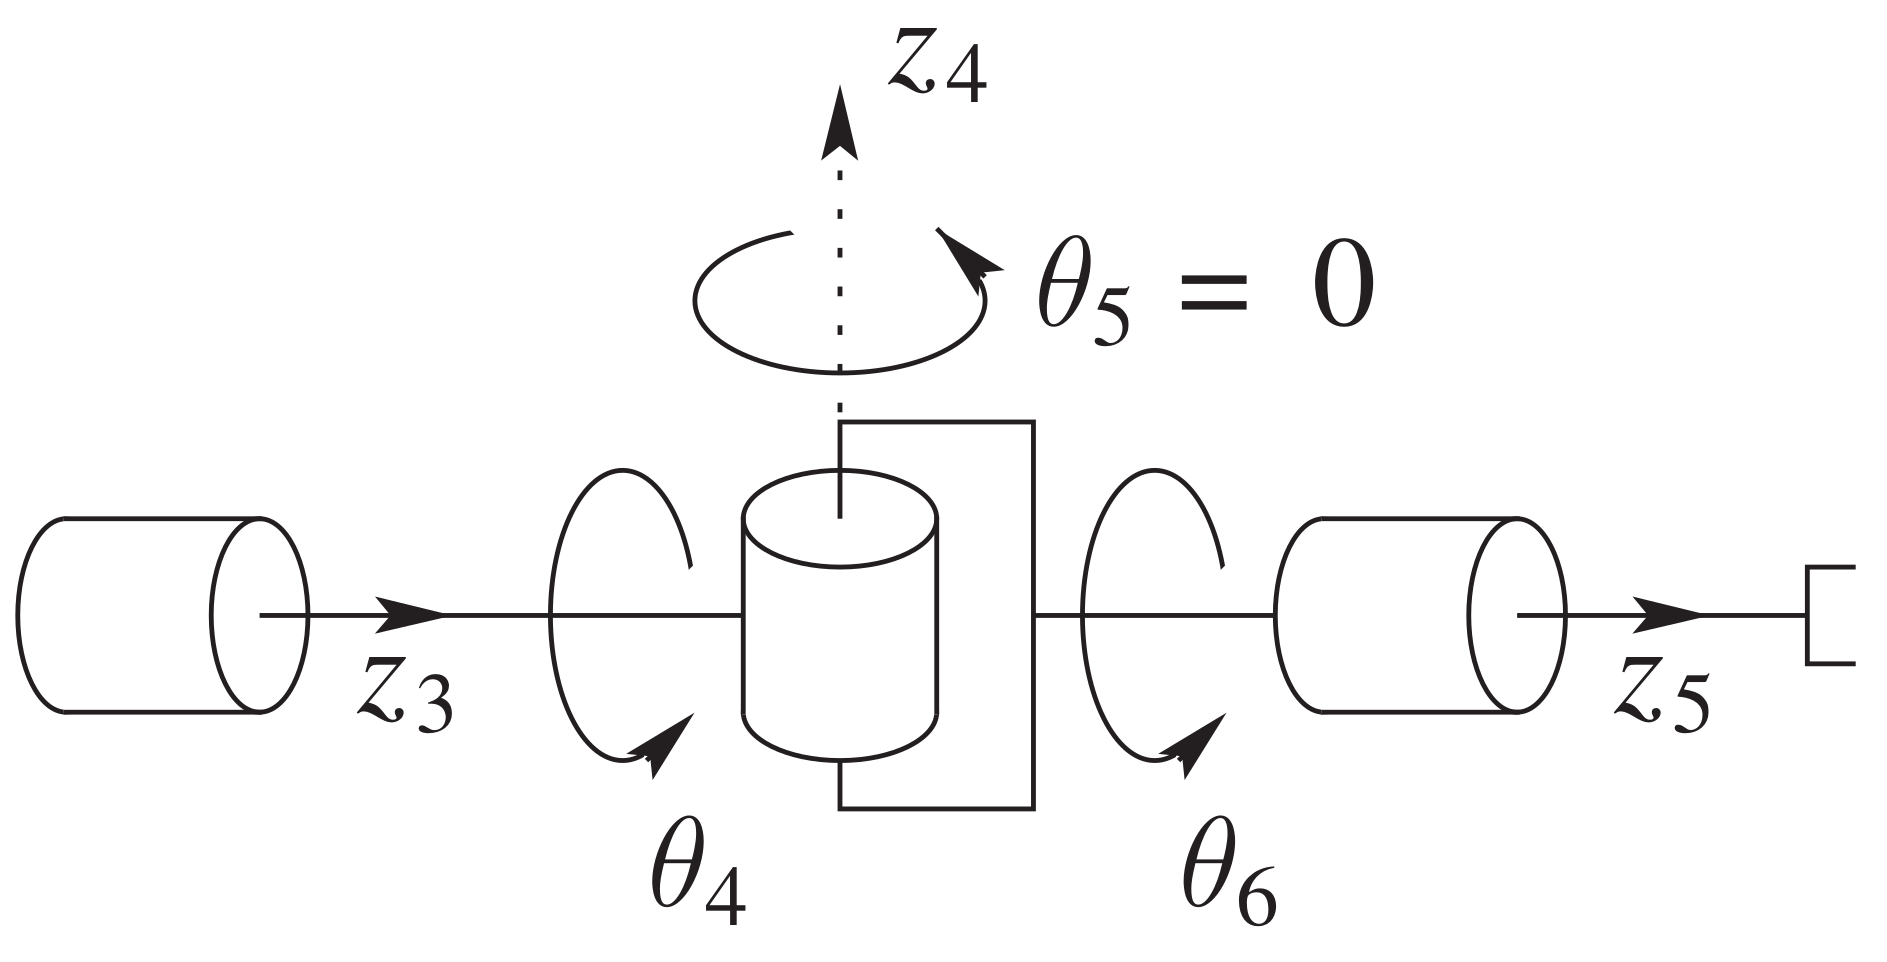
\includegraphics[width=0.85\textwidth]{figures/spherical_wrist_singularity.png} 
                % \caption{\footnotesize }
            \end{figure}
            \vspace{-2mm}
            \centering
            \footnotesize{Spherical wrist singularity}
        \end{column}
    \end{columns}
\end{frame}



\begin{frame}
    \frametitle{Arm Singularities}

    \begin{itemize}
        \item To investigate arm singularities we need only to compute $\det
        J_{11}$, which is done using the equation
        \[ J_{v_i} = 
        \begin{cases}
            z_{i-1} \times (o - o_{i-1}) & \mbox{for revolute joint $i$} \\
            z_{i-1} & \mbox{for prismatic joint $i$}
        \end{cases}    
        \]
        where $o$ is the wrist center.
    \end{itemize}
\end{frame}


\begin{frame}
    \frametitle{Arm Singularities of Elbow Manipulator}

    \begin{itemize}
        \item The three-link articulated manipulator has the determinant $J_{11}$
        \[
            J_{11} = \bmat{
                -a_2s_1c_2 - a_3s_1c_{23} & -a_2s_2c_1 - a_3s_{23}c_1 & -a_3c_1s_{23} \\ 
                a_2c_1c_2 + a_3c_1c_{23} & -a_2s_1s_2 - a_3s_1s_{23} & -a_3s_1s_{23} \\ 
                0 & a_2c_2 + a_3c_{23} & a_3c_{23}
            }
        \]
    \end{itemize}
    \begin{columns}
        \begin{column}{0.6\textwidth}
            \begin{itemize}
                \item The determinant of $J_{11}$ is 
                \[ \det J_{11} = -a_2a_3s_3(a_2c_2 + a_3c_{23}). \]
            \end{itemize}
        \end{column}
        \begin{column}{0.4\textwidth}
            \begin{figure}[bth]
                \centering
                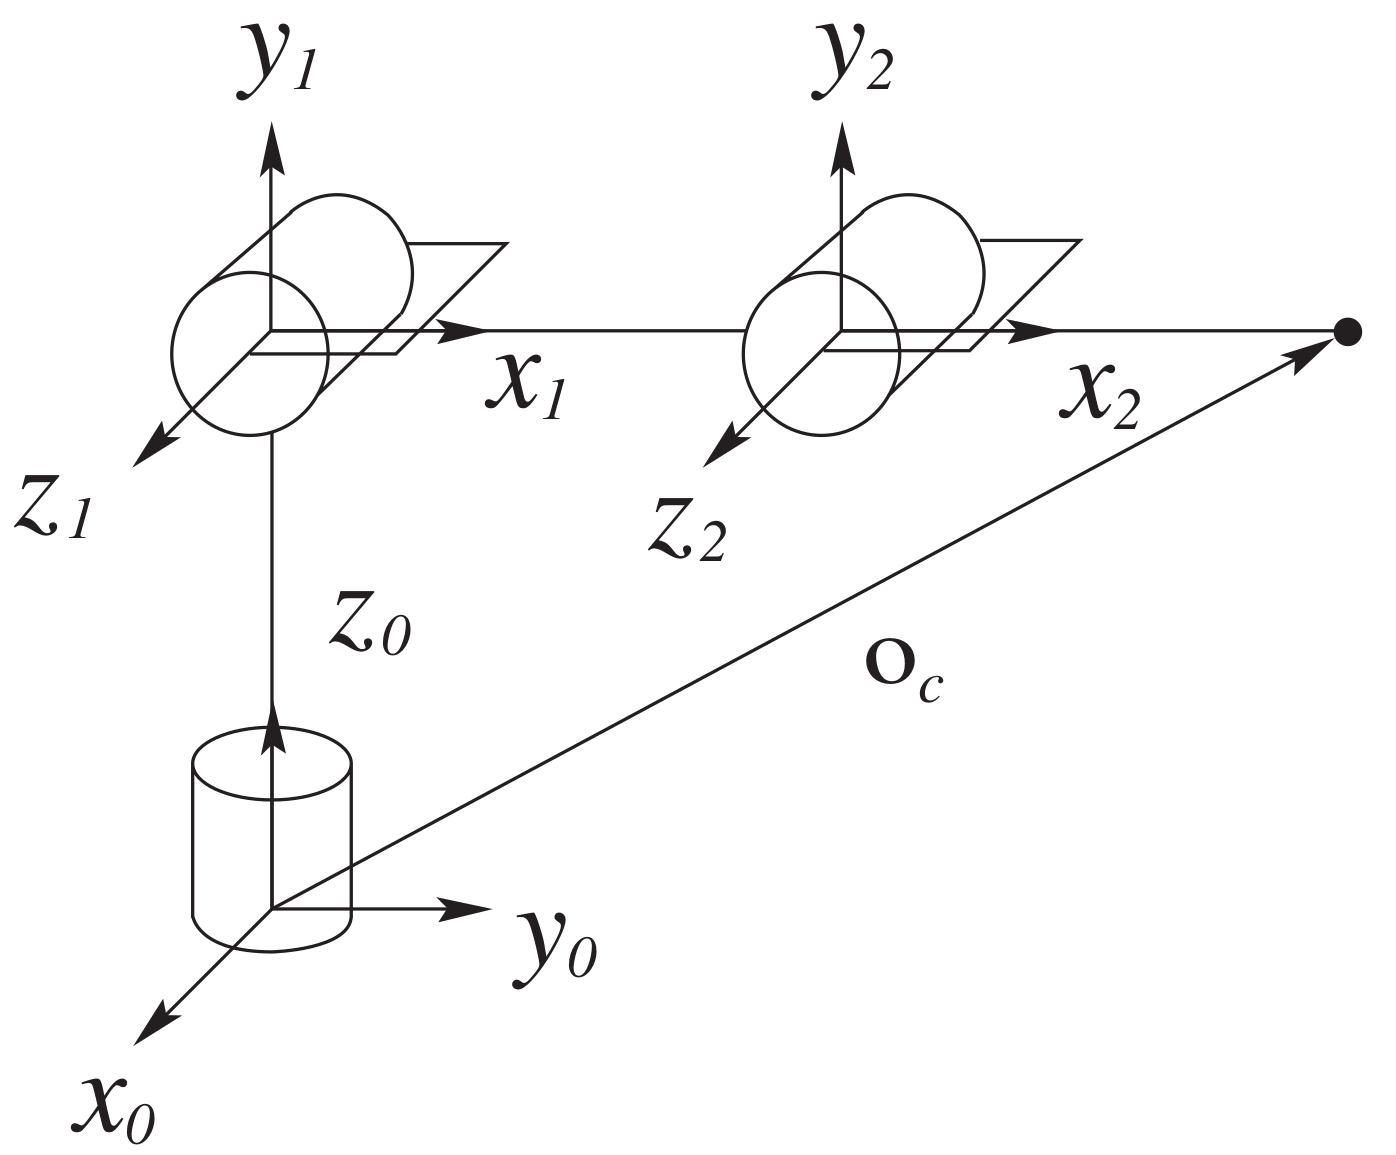
\includegraphics[width=0.85\textwidth]{figures/elbow_manipulator_sing.png} 
                % \caption{\footnotesize }
            \end{figure}
            \vspace{-2mm}
            \centering
            \footnotesize{Elbow manipulator}
        \end{column}
    \end{columns}
\end{frame}


\begin{frame}
    \frametitle{Arm Singularities of Elbow Manipulator}

    \begin{columns}
        \begin{column}{0.6\textwidth}
            \begin{itemize}
                \item We see that the elbow manipulator is
                in a singular configuration when
                \[ s_3 = 0 \Longrightarrow \theta_3 = 0, \pi. \]
                and whenever
                \[ a_2c_2 + a_3c_{23} = 0. \]
                \item The situation of $\theta_3 = 0, \pi$ arises when the elbow
                is fully extended or retracted as shown on the bottom right
                figure.
            \end{itemize}
        \end{column}
        \begin{column}{0.4\textwidth}
            \begin{figure}[bth]
                \centering
                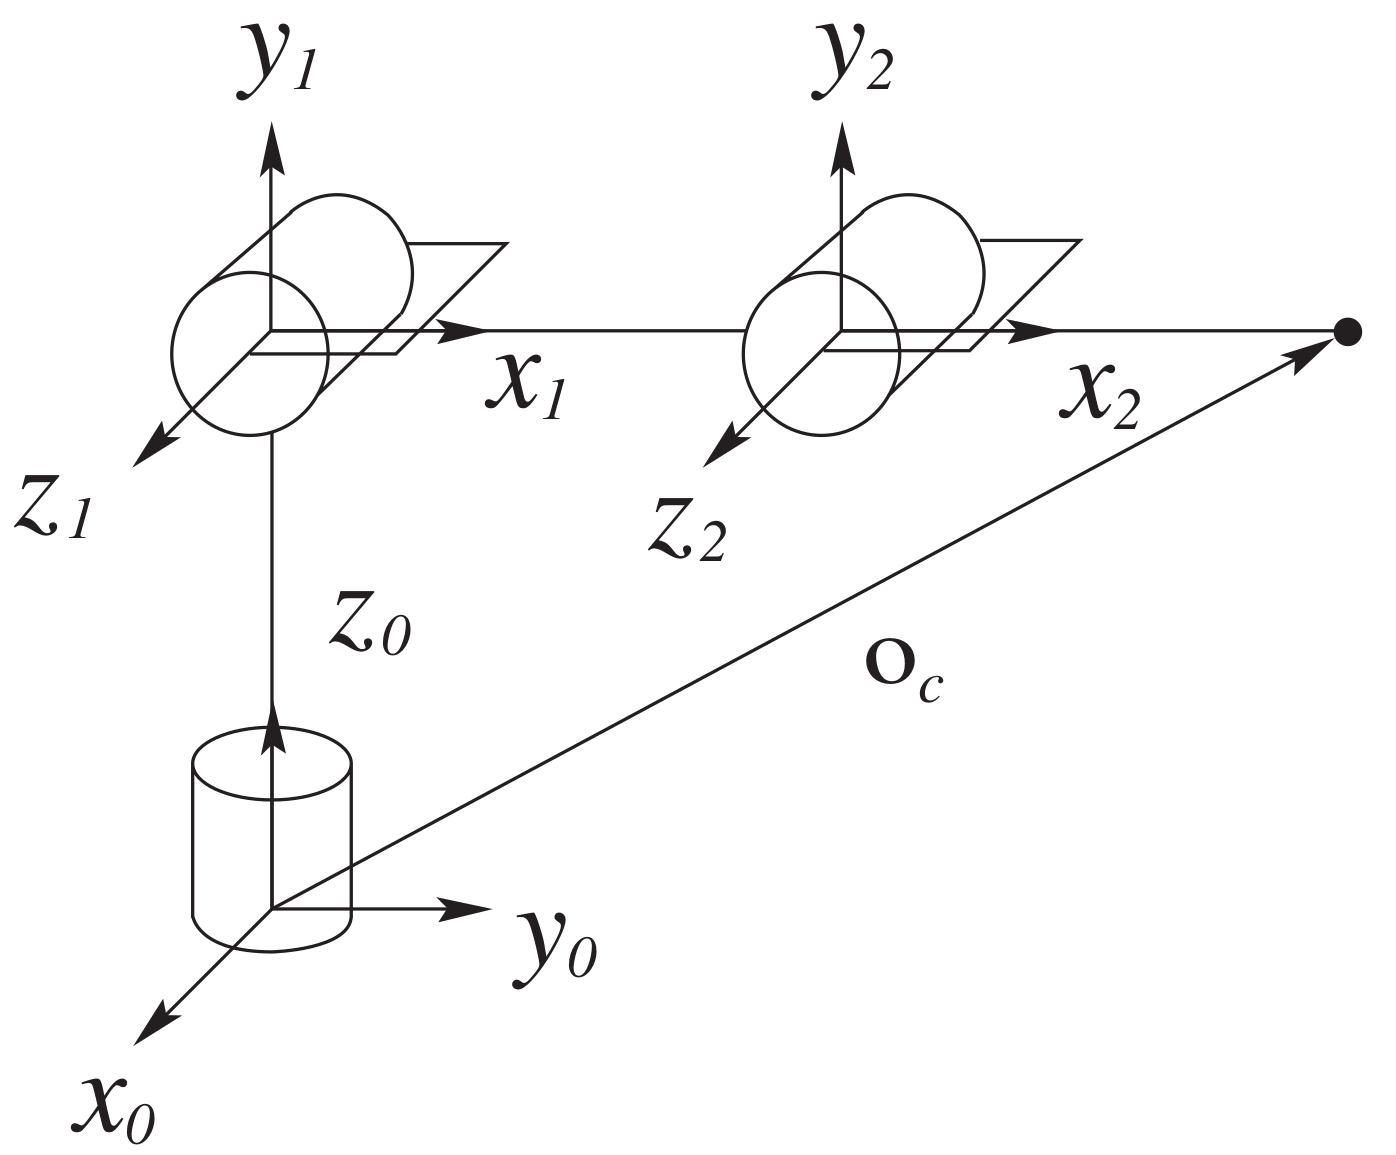
\includegraphics[width=0.85\textwidth]{figures/elbow_manipulator_sing.png} 
                % \caption{\footnotesize }
            \end{figure}
            \vspace{-2mm}
            \centering
            \footnotesize{Elbow manipulator}

            \begin{figure}[bth]
                \centering
                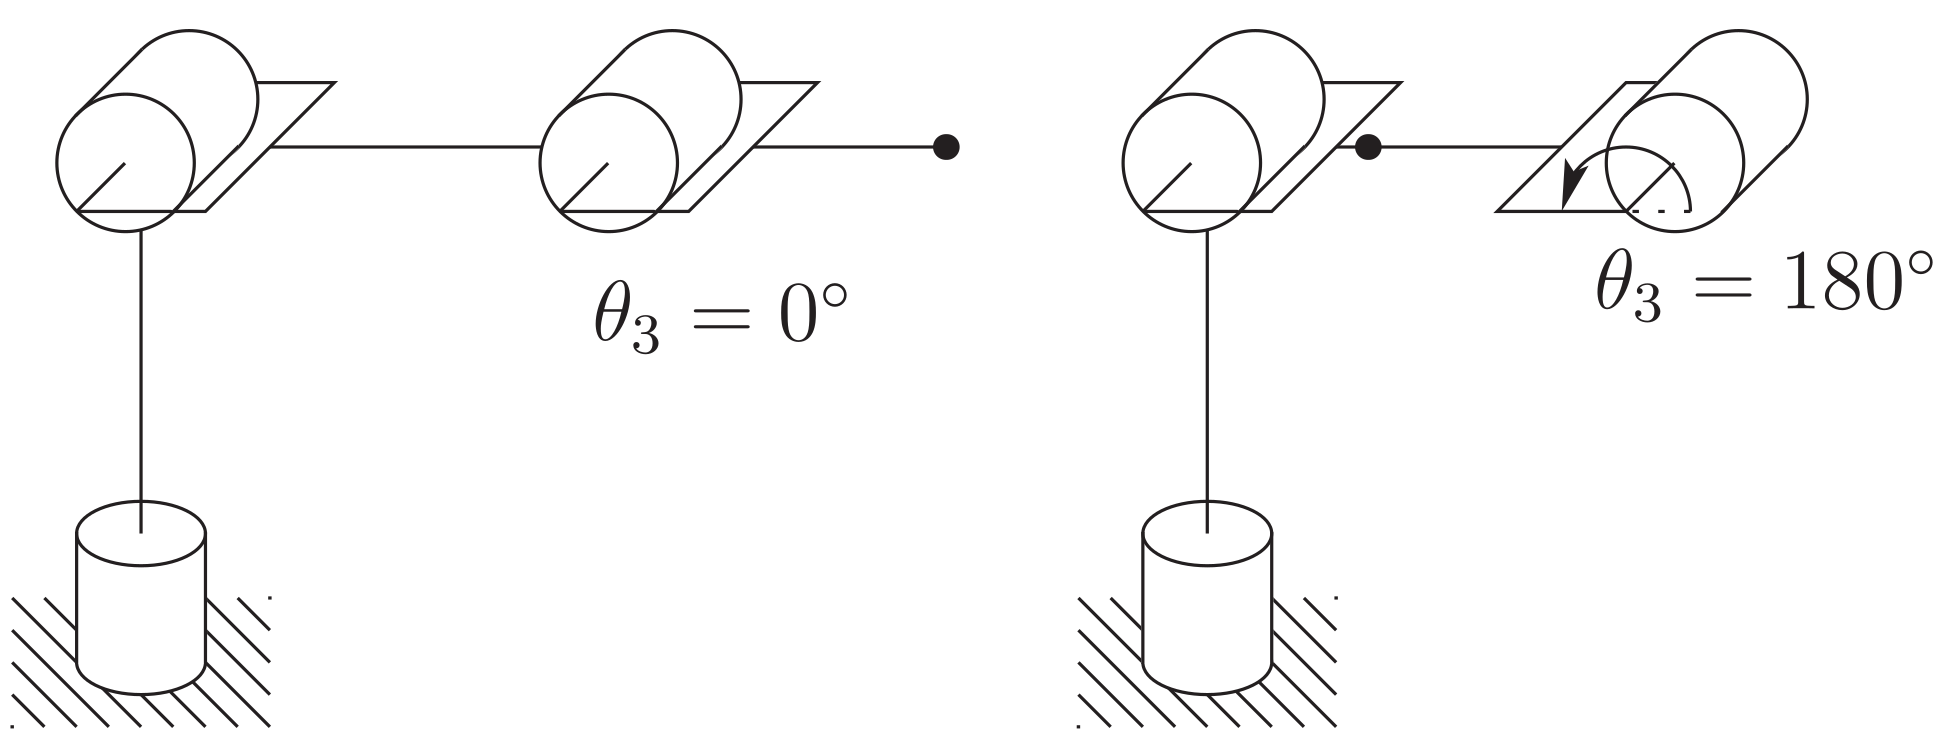
\includegraphics[width=0.85\textwidth]{figures/elbow_singularities.png} 
                % \caption{\footnotesize }
            \end{figure}
            \vspace{-2mm}
            \centering
            \footnotesize{Elbow singularities of the elbow manipulator}
        \end{column}
    \end{columns}
\end{frame}


\begin{frame}
    \frametitle{Arm Singularities of Elbow Manipulator}

    \begin{columns}
        \begin{column}{0.6\textwidth}
            \begin{itemize}
                \item The situation of 
                \[ a_2c_2 + a_3c_{23} = 0. \]
                is shown on the top right figure.
                \item This configuration occurs when the wrist center intersects
                the axis of the base rotation, $z_0$.
                \item If the elbow manipulator has an offset (bottom right
                figure), the wrist center cannot intersect $z_0$.
            \end{itemize}
        \end{column}
        \begin{column}{0.4\textwidth}
            \begin{figure}[bth]
                \centering
                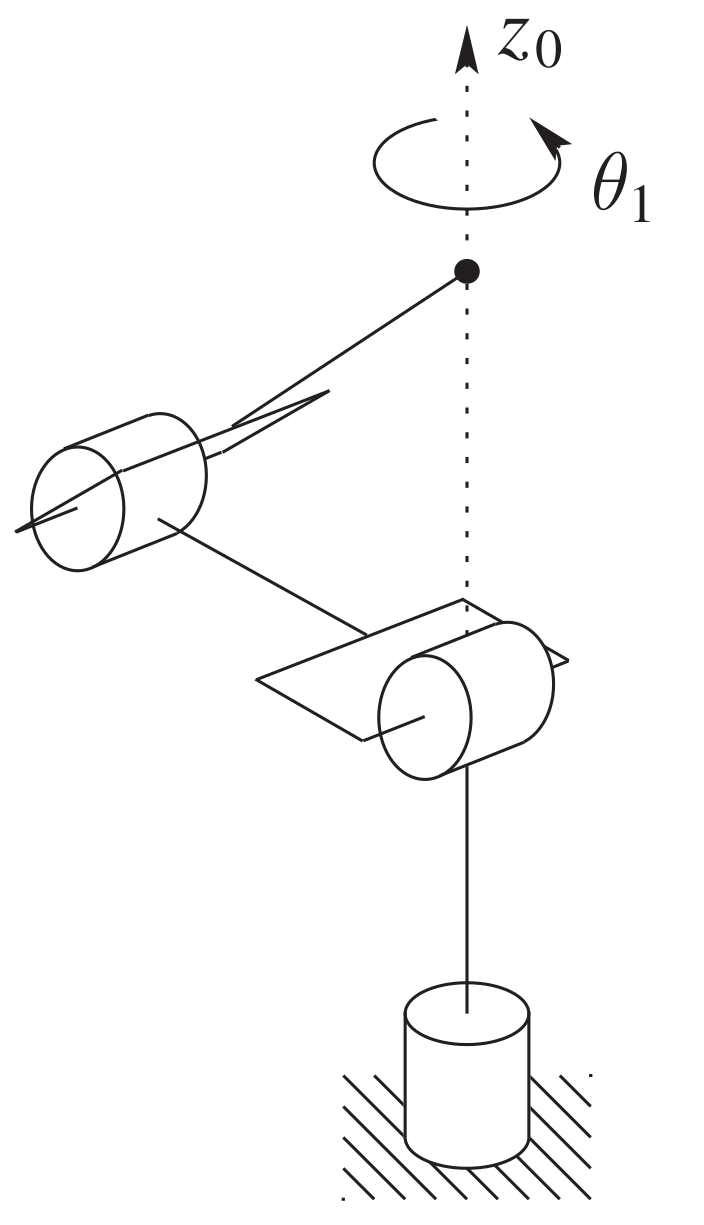
\includegraphics[width=0.4\textwidth]{figures/elbow_sing_no_offset.png} 
                % \caption{\footnotesize }
            \end{figure}
            \vspace{-2mm}
            \centering
            \footnotesize{Singularity of elbow manipulator with no offsets.}

            \begin{figure}[bth]
                \centering
                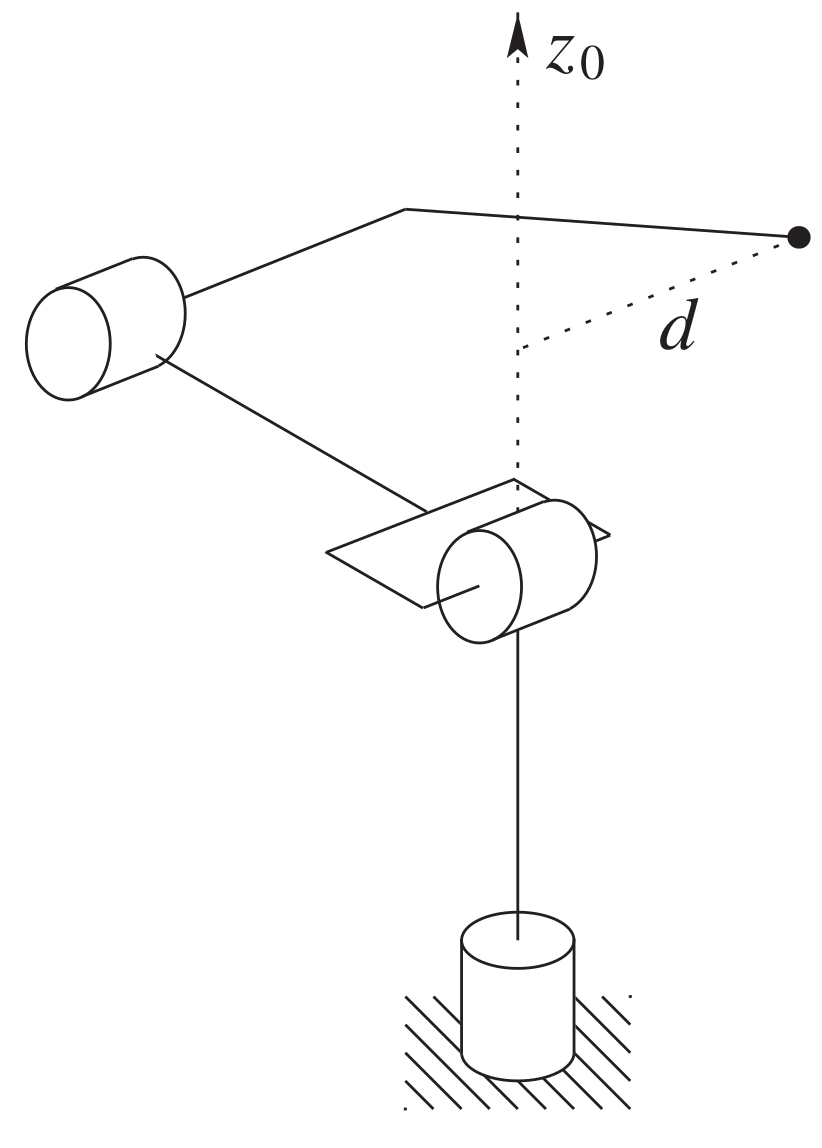
\includegraphics[width=0.4\textwidth]{figures/elbow_sing_w_offset.png} 
                % \caption{\footnotesize }
            \end{figure}
            \vspace{-2mm}
            \centering
            \footnotesize{Elbow manipulator with an offset at the elbow.}
        \end{column}
    \end{columns}
\end{frame}


\endgroup
% \section{Static Force/Torque Relationships}

\begin{frame}[standout, plain, noframenumbering]
    Static Force/Torque Relationships

    % \medskip

    % \footnotesize
    % Sam Greydanus \quad Misko Dzamba \quad Jason Yosinski
\end{frame}

\begingroup
\small


\begin{frame}
    \frametitle{Static Force/Torque Relationships}

    \begin{itemize}
        \item Interaction of the manipulator with the environment produces
        forces and moments at the end effector or tool.
        \item These produce torques at the joints of the robot.\footnotemark
        \item We discuss the role of the manipulator Jacobian in the
        quantitative relationship between the end effector forces and joint
        torques.
        \item Let $F = (F_x, F_y, F_z, n_x, n_y, n_z)$ represent the vector of 
        forces and moments at the end effector.
        \item Let $\tau$ denote the corresponding vector of joint torques. Then 
        \begin{equation}
            \boxed{\tau = J^\top(q) F.}
            \label{eq:static_force_torque}
        \end{equation} 
    \end{itemize}

    \footnotetext{We consider only revolute joints. If the joints are prismatic, 
    forces and moments at the end effector produce forces at the joints.}
\end{frame}


\begin{frame}
    \frametitle{Static Force/Torque Relationships}

    \begin{itemize}
        \item We derive the relationship~\eqref{eq:static_force_torque} through 
        the so-called \textbf{principle of virtual work}.
        \item Its detailed discussion is deferred. Instead an informal
        justification follows.
        \item Let $\delta X$ and $\delta q$ represent infinitesimal
        displacements in the task space and joint space, respectively.
        \item These displacements are called \textbf{virtual displacements} if 
        they are consistent with any constraints imposed on the system.
        \item For example, if the end effector is in contact with a rigid wall, 
        then the virtual displacements in position are tangent to the wall.
        \item These virtual displacements are related through the manipulator 
        Jacobian $J(q)$ according to 
        \begin{equation}
            \delta X = J(q) \delta q.
            \label{eq:virtual_displacement}
        \end{equation}
    \end{itemize}
\end{frame}


\begin{frame}
    \frametitle{Static Force/Torque Relationships}

    \begin{itemize}
        \item The virtual work $\delta w$ of the system is 
        \[ \delta w = F^\top \delta X - \tau^\top \delta q. \]
        \item Substituting equation~\eqref{eq:virtual_displacement} into the
        equation above yields
        \begin{equation}
            \delta w = \left( F^\top J - \tau^\top \right) \delta q.
            \label{eq:force_torque}
        \end{equation} 
        \item The principle of virtual work says that the quantity given by
        equation~\eqref{eq:force_torque} is equal to zero if the manipulator is
        in equilibrium. This gives rise to the
        equation~\eqref{eq:static_force_torque}.
    \end{itemize}
\end{frame}



\begin{frame}
    \frametitle{Example: Two-Link Planar Manipulator}

    \begin{columns}
        \begin{column}{0.6\textwidth}
            \begin{itemize}
                \item A force $F$ is applied at the end of link $2$ as shown.
                \item The Jacobian of this manipulator was formulated earlier.
                \item The resulting joint torques $\tau = (\tau_1, \tau_2)$ are 
                then given by 
            \end{itemize}
        \end{column}
        \begin{column}{0.4\textwidth}
            \begin{figure}[bth]
                \centering
                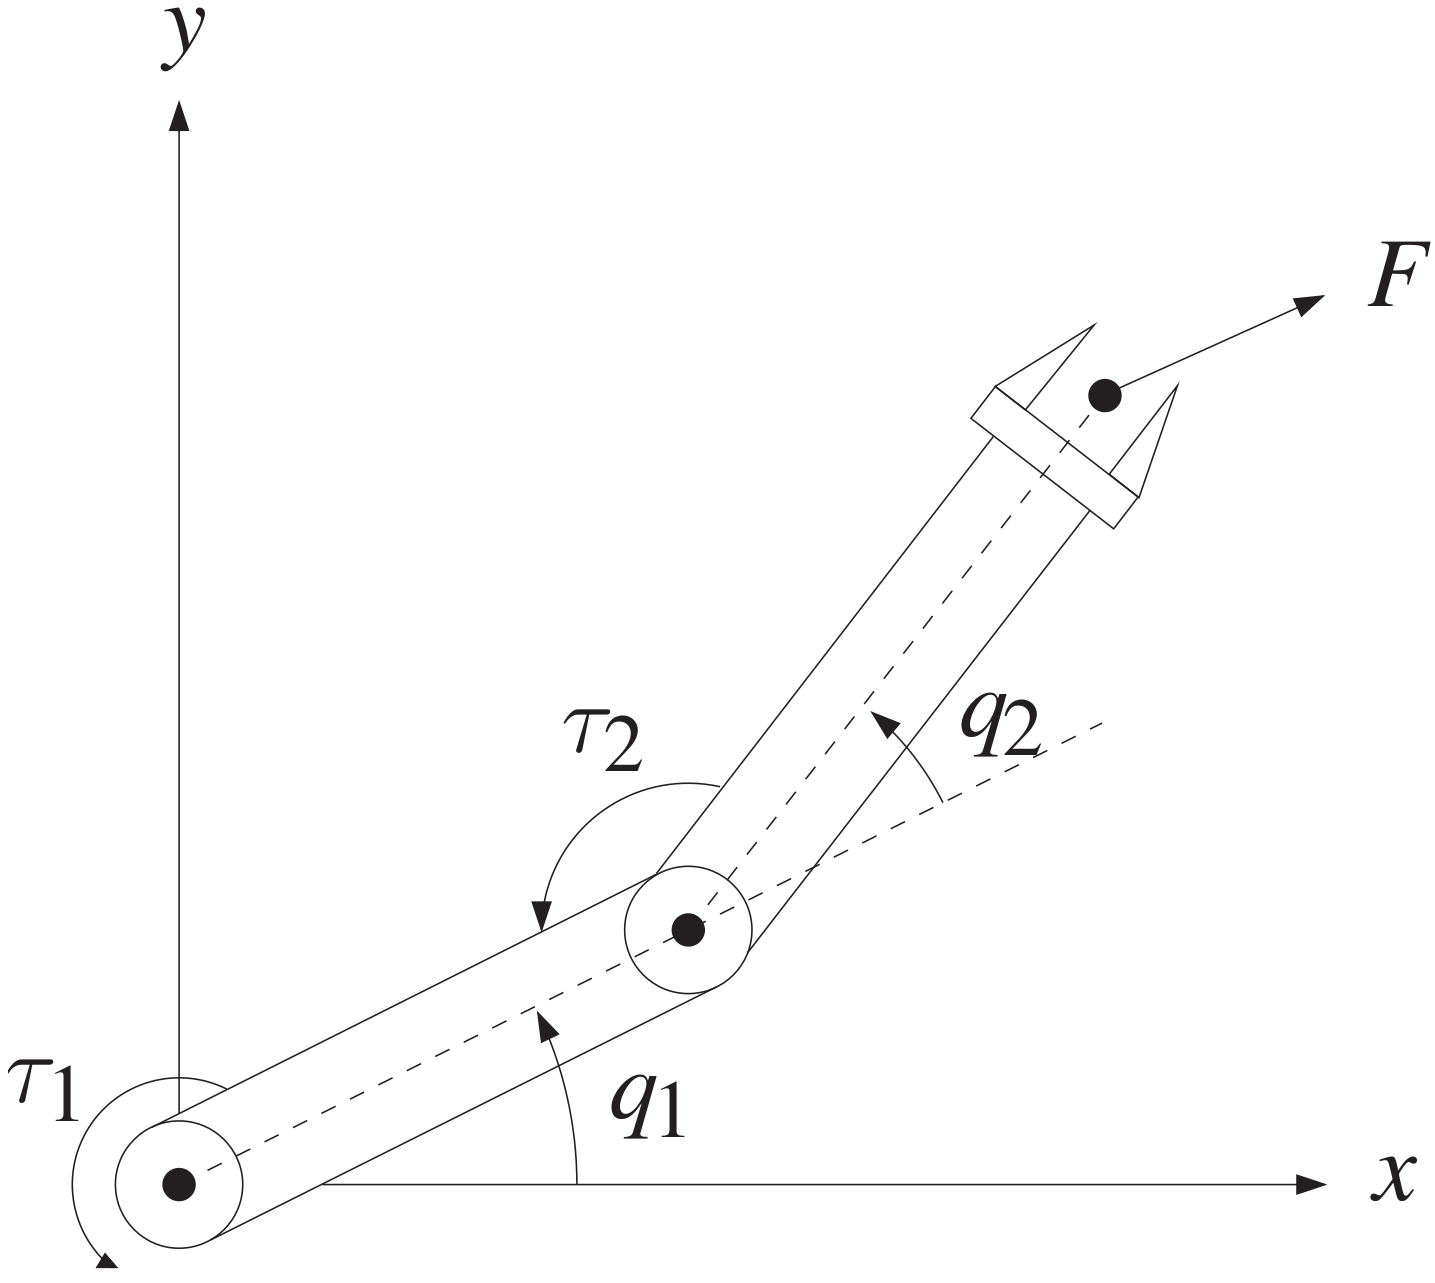
\includegraphics[width=0.85\textwidth]{figures/two_link_robot.png} 
                % \caption{\footnotesize }
            \end{figure}
            \vspace{-2mm}
            \centering
            \footnotesize{Two-link planar robot.}
        \end{column}
    \end{columns}
    \[
    \bmat{\tau_1 \\ \tau_2} = \bmat{
        -a_1s_1 - a_2s_{12} & a_1c_1 + a_2c_{12} & 0 & 0 & 0 & 1 \\ 
        -a_2s_{12} & a_2c_{12} & 0 & 0 & 0 & 1
    }\bmat{F_x \\ F_y \\ F_z \\ n_x \\ n_y \\ n_z}.
    \]
\end{frame}


\endgroup
% \section{Inverse Velocity and Acceleration}

\begin{frame}[standout, plain, noframenumbering]
    Inverse Velocity and Acceleration

    % \medskip

    % \footnotesize
    % Sam Greydanus \quad Misko Dzamba \quad Jason Yosinski
\end{frame}

\begingroup
\small


\begin{frame}
    \frametitle{Inverse Velocity and Acceleration}

    \begin{itemize}
        \item The inverse velocity problem is the problem of finding the joint
        velocities $\dot{q}$ that produce the desired end effector velocity by
        solving the equation
        \begin{equation}
            \xi = J\dot{q}
            \label{eq:vel}
        \end{equation}
        \item When the Jacobian is square and nonsingular, this problem can be 
        solved by simply inverting the Jacobian matrix, to give \[\dot{q} = J^{-1}\xi. \]
        \item For manipulators that do not have exactly six joints, the Jacobian
        cannot be inverted. In this case, there will be a solution to
        equation~\eqref{eq:vel} if and only if $\xi$ lies in the range space of
        the Jacobian. This is the case if and only if \[ \rank{J(q)} = \rank
        \hspace{-6mm} \underbrace{\bmat{J(q) | \xi}}_{\textrm{augmented matrix}}
        \hspace{-6mm}. \]
    \end{itemize}
\end{frame}


\begin{frame}
    \frametitle{Inverse Velocity and Acceleration}

    \begin{itemize}
        \item If $n > 6$, we can solve for $\dot{q}$ using the right
        pseudoinverse of $J$. Problem 4-20 shows that a solution to
        equation~\eqref{eq:vel} is given by 
        \[ \dot{q} = J^\dagger \xi + (I - J^\dagger J)b, \] in which $b \in
        \mathbb{R}^n$ is an arbitrary vector.
        \item For $m < n$, $(I - J^\dagger J) \neq 0$, and all vectors of the
        form $(I - J^\dagger J)b$ lie in the nullspace of $J$.
        \begin{itemize}
            \footnotesize{
            \item If $\dot{q}^' = (I - J^\dagger J)b$, then when the joints move 
            with velocity $\dot{q}^'$, the end effector will remain fixed since 
            $J\dot{q}^' = 0$.
            \item Thus, if $\dot{q}$ solves eqn.~\eqref{eq:vel}, then so does 
            $\dot{q} + \dot{q}^'$ with $\dot{q}^' = (I - J^\dagger J)b$, for any 
            vector $b \in \mathbb{R}^3$.
            \item If the goal is to minimize the resulting joint velocities, we 
            choose $b = 0$ (Problem 4-20).
            }
        \end{itemize}
    \end{itemize}
\end{frame}


\endgroup
% \section{Manipulability}

\begin{frame}[standout, plain, noframenumbering]
    Manipulability

    % \medskip

    % \footnotesize
    % Sam Greydanus \quad Misko Dzamba \quad Jason Yosinski
\end{frame}

\begingroup
\small


\begin{frame}
    \frametitle{Manipulability}

    \begin{itemize}
        \item For a specific configuration $q$, the Jacobian relationship
        defines the linear system given by $\xi = J\dot{q}$.
        \item We can think of $J$ as scaling the input $\dot{q}$ to produce the 
        output $\xi$.
        \item We want to characterize the output in terms of an input that has
        unit norm. Consider the set of all robot joint velocities $\dot{q}$ s.t.
        \[ \norm{\dot{q}}{}^2 = \dot{q}_1^2 + \dot{q}_2^2 + \cdots + \dot{q}_n^2 \leq 1. \]
        \item If we use the minimum norm solution $\dot{q} = J^\dagger \xi$, we
        obtain 
        \begin{equation}
            \norm{\dot{q}}{}^2 = \dot{q}^\top \dot{q} = \left( J^\dagger
        \xi \right)^\top J^\dagger \xi = \xi^\top \left( JJ^\top
        \right)^{-1}\xi.
        \label{eq:jac_scaling}
        \end{equation} 
        \item Equation~\eqref{eq:jac_scaling} gives us a quantitative
        characterization of the scaling effected by the Jacobian.
        \item If $\rank J = m$, then eqn.~\eqref{eq:jac_scaling} defines an
        $m$-dimensional ellipsoid that is known as the \textbf{manipulability
        ellipsoid}. 
    \end{itemize}
\end{frame}



\begin{frame}
    \frametitle{Manipulability}

    \begin{itemize}
        \item If the input (joint velocity) vector has unit norm, then the
        output (end-effector velocity) will lie within the ellipsoid given by 
        equation~\eqref{eq:jac_scaling}.
        \item Perfoming a singular value decomposition (SVD) of $J = U\Sigma
        V^\top$ we see that
        \[ \xi^\top \left(JJ^\top\right)^{-1}\xi = \left( U^\top \xi
        \right)^\top \Sigma_m^{-2}\left( U^\top \xi \right) \] in which 
        \[
        \Sigma_m^{-2} = \bmat{
            \sigma_1^{-2} & & & \\
            & \sigma_2^{-2} & & \\
            & & \ddots & \\
            & & & \sigma_m^{-2}
        },
        \] and $\sigma_1 \geq \sigma_2 \geq \cdots \geq \sigma_m \geq 0$.
    \end{itemize}
\end{frame}


\begin{frame}
    \frametitle{Manipulability}

    \begin{itemize}
        \item If we make the substitution $w = U^\top \xi$, then the equation in
        the previous slide becomes \[ w^\top \Sigma_m^{-2}w = \sum
        \frac{w_i^2}{\sigma_i^2} \geq 1, \] and it is clear that this is the
        equation for an axis-aligned ellipsoid in a new coordinate system that
        is obtained by rotation according to the orthogonal matrix $U^\top$.
        \item In the original coordinate system, the axes of the ellipsoid are
        given by the vectors $\sigma_i u_i$.
        \item The volume of the ellipsoid is given by
        \[ \textrm{volume} = K\sigma_1\sigma_2 \cdots \sigma_m, \] in which $K$
        is a constant that depends only on the dimension $m$ of the ellipsoid.
    \end{itemize}
\end{frame}

\begin{frame}
    \frametitle{Manipulability}
    
    \begin{itemize}
        \item The manipulability measure is given by \[ \mu =
        \sigma_1\sigma_2\cdots\sigma_m. \]
        \item Now, let's consider the special case when the robot is not
        redundant, that is, $J \in \mathbb{R}^{m \times m}$.
        \item Recall that the determinant of a product is equal to the product
        of the determinants, and that a matrix and its transpose have the same
        determinant. Thus, \[ \det JJ^\top = \lambda_1^2 \lambda_2^2 \cdots
        \lambda_m^2, \] in which $\lambda_1 \geq \lambda_2 \geq \cdots \geq
        \lambda_m$ are the eigenvalues of $J$. This leads to
        \[ \mu = \sqrt{\det JJ^\top} = \abs{\lambda_1 \lambda_2 \cdots \lambda_m} = \abs{\det J}. \]
    \end{itemize}
\end{frame}


\begin{frame}
    \frametitle{Manipulability ($\mu$) Properties}

    \begin{itemize}
        \item In general, $\mu = 0$ holds iff $\rank J < m$, i.e., when $J$ is
        not full rank.
        \item Suppose that there is some error in the measured velocity $\Delta
        \xi$. We can bound the corresponding error in the computed joint
        velocity $\Delta \dot{q}$ by \[ \left( \sigma_1 \right)^{-1} \leq
        \frac{\norm{\Delta \dot{q}}{}}{\norm{\Delta \xi}{}} \leq \left( \sigma_m
        \right)^{-1} \]
    \end{itemize}
\end{frame}


\begin{frame}
    \frametitle{Two-link Arm Manipulability}

    \begin{columns}
        \begin{column}{0.6\textwidth}
            \begin{itemize}
                \item The Jacobian is given by 
                \[
                J = \bmat{
                    -a_1s_1 - a_2s_{12} & -a_2s_{12} \\ 
                    a_1c_1 + a_2c_{12} & a_2c_{12}
                }
                \]
                and the manipulability is given by \[\mu = \abs{\det J} = a_1a_2\abs{s_2}.  \]
                \only<1>{
                \item Manipulability can be used to determine optimal
                configurations in which to perform certain tasks.
                \item It may be desirable to perform a task in the configuration
                for which the end effector has the maximum manipulability
                ($\theta_2 = \pm \frac{\pi}{2}$).
                }
                \onslide<2->{
                \item Manipulability can also be used to aid in the design of 
                manipulators.
                \item Suppose that we wish to design a two-link arm whose total
                link length $a_1 + a_2$ is fixed. What values should we choose for $a_1$ and $a_2$?
                }
            \end{itemize}
        \end{column}
        \begin{column}{0.4\textwidth}
            \begin{figure}[bth]
                \centering
                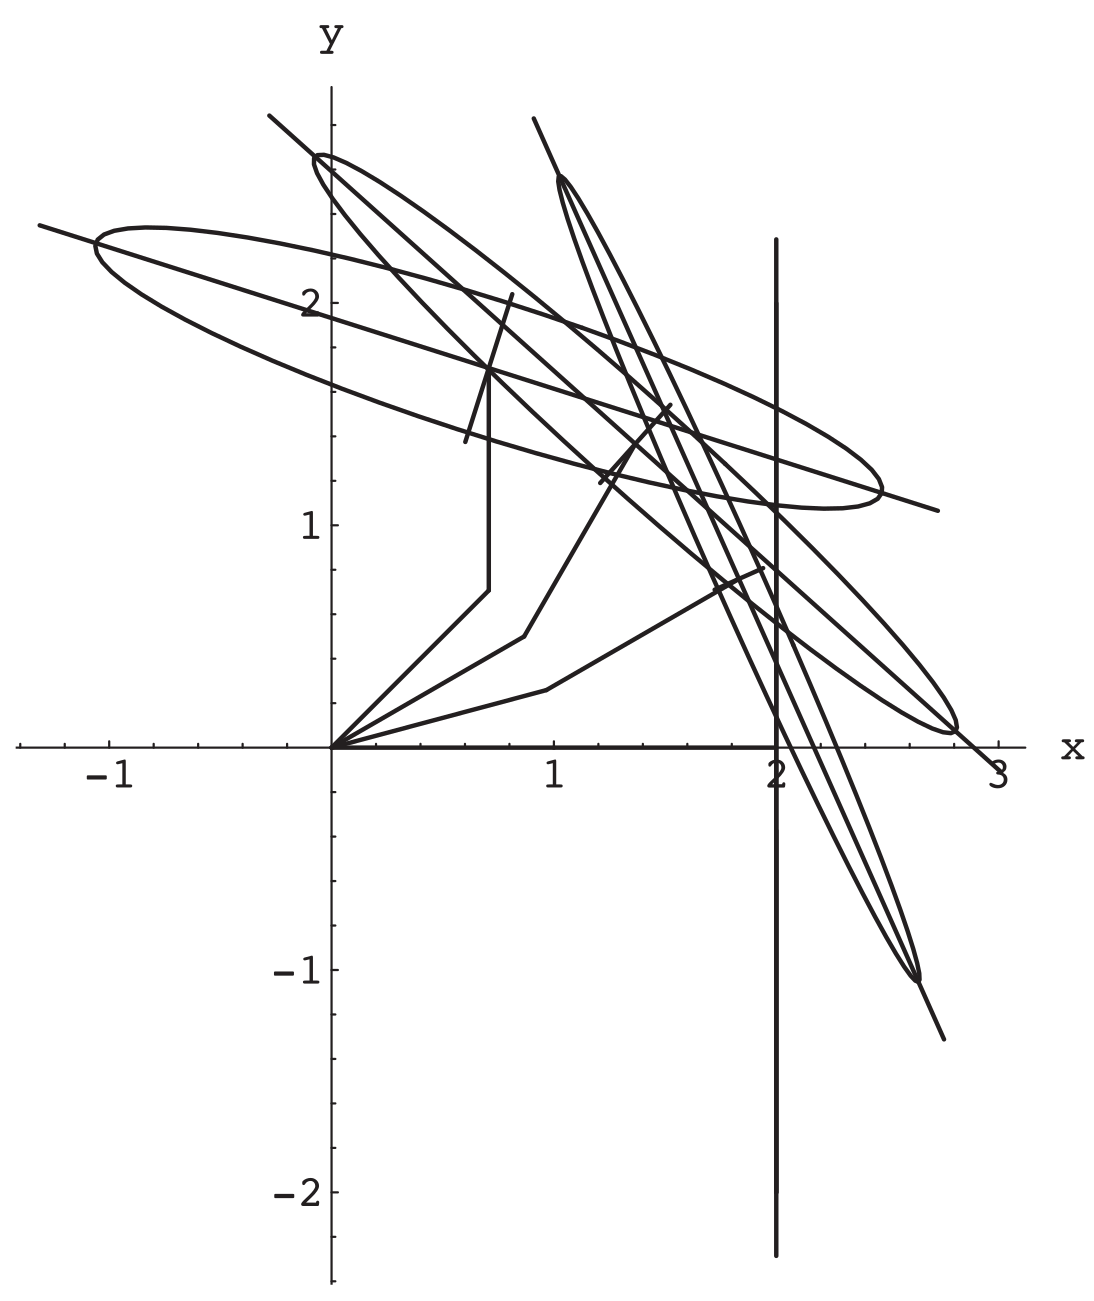
\includegraphics[width=0.85\textwidth]{figures/manipulability_ellipsoids_two_link.png} 
                % \caption{\footnotesize }
            \end{figure}
            \vspace{-2mm}
            \centering
            \footnotesize{Singularity of elbow manipulator with no offsets.}

            \vspace{3mm}
            \only<3>{
            \begin{itemize}
                \item Choose them such that the manipulability $\mu$ is maximized: $a_1 = a_2$.
            \end{itemize}
            }
        \end{column}
    \end{columns}
\end{frame}


\endgroup


%------------------------------------------------
%   The Bibliography
%------------------------------------------------
% \begin{frame}
%     \frametitle{References}
%     \bibliographystyle{abbrvnat}
%     \bibliography{wankun_thesis}
% \end{frame}

%------------------------------------------------
%   The End
%------------------------------------------------
\begin{frame}[plain, standout, noframenumbering]\end{frame}
% \appendix

\section{Similarity Transformations}

\begin{frame}[standout, plain, noframenumbering]
    Appendix

    % \medskip

    % \footnotesize
    % Sam Greydanus \quad Misko Dzamba \quad Jason Yosinski
\end{frame}

\begin{frame}
    \frametitle{Similarity Transformations -- Detailed}

    \begin{block}{Coordinate Isomorphism}
        Let $V$ be a vector space over $\mathbb{R}$ and $\mc{F} = \{f_1, \ldots,
        f_n \}$ be a basis of $V$.

        If $v \in V$, then $v = a_1f_1 + \cdots + a_n f_n$, where $a_i \in
        \mathbb{R}$ for $i = 1, \ldots, n$ are the \textit{coordinates} of $v$
        relative to $\mc{F}$. 
        
        The vector $a = \bmat{a_1 & \cdots & a_n}^\top \in
        \mathbb{R}^n$ is called the \textit{coordinate tuple} of $v$ relative to
        $\mc{F}$.

        The unique linear map $\varphi: \mathbb{R}^n \rightarrow V$ with
        $\varphi(e_j) = f_j$ for $j = 1, \ldots, n$ is called the
        \textbf{coordinate isomorphism} for $V$ and the basis $\mc{F}$. Here
        $e_j$ is the $j^{\textrm{th}}$ standard basis of $\mathbb{R}^n$.

        Thus $\varphi(a) = v$ if and only if $v = a_1 f_1 + \cdots + a_n f_n$.
    \end{block}
\end{frame}


\begin{frame}
    \frametitle{Similarity Transformations -- Detailed}

    \begin{block}{The matrix of a linear transformation}
        Let $T \in \End(V)$, i.e., $T: V \rightarrow V$ is a linear operator.
        
        The map $A = \varphi^{-1} \circ T \circ \varphi \in \End \mathbb{R}^n$
        and therefore has a matrix $[A]$; its $j^{\textrm{th}}$ column is
        $\varphi^{-1}(T(f_j))$ for $j = 1, \ldots, n$. This matrix is called the
        matrix of $T$ w.r.t. the basis $\mc{F}$.

        If $V \ni \tilde{v} = T(v)$ and $b$ and $a$ are the coordinate tuples of 
        $\tilde{v}$ and $v$, then $b = \varphi^{-1}\left(T(\varphi(a))\right) = 
        [A]a$. 

        Conversely, if $v \in V$ and $a = \varphi^{-1}(v)$ is the coordinate
        tuple of $v$ w.r.t. $\mc{F}$, and we set $b = [A]a$ and $\tilde{v} =
        \varphi(b)$, then $\tilde{v} = \varphi(A(a)) = T(v)$. That is $b = [A]a$ 
        if and only if $\tilde{v} = T(v)$.
    \end{block}
    
\end{frame}

\begin{frame}
    \frametitle{Similarity Transformations -- Detailed}

    \begin{block}{Theorem 1: Composition of linear transformations}
        Suppose $U$, $V$, and $W$ are vector spaces of finite dimension and a
        basis is chosen for each. 
        
        If $T \in \Hom(U, V)$ and $S \in Hom(V, W)$ with matrices $[A]$ and
        $[B]$, then the matrix of the linear transformation $S \circ T \in
        \Hom(U, W)$ w.r.t. the given bases is $[A][B]$.
    \end{block}
\end{frame}


\begin{frame}
    \frametitle{Similarity Transformations -- Detailed}

    Let $\mc{F} = \{f_1, \ldots, f_n \}$ and $\mc{F}^' = \{f_1^', \ldots,
    f_n^'\}$ be two bases for $V$. Let $\varphi$ and $\varphi^'$ be the
    coordinate isomorphisms, taking the standard basis in $\mathbb{R}^n$ to the
    first and second bases for $V$.

    Let $A = \varphi^{-1} \circ T \circ \varphi$, $B =
    {\left(\varphi^'\right)}^{-1} \circ T \circ {\varphi^'}$, $P = \varphi^{-1}
    \circ \varphi^'$ and $[P]$ be the matrix of $P: \mathbb{R}^n \rightarrow
    \mathbb{R}^n$. This means that element $(k,j)$, $p_{kj}$, of $[P]$ is found
    from 
    \vspace{-2mm}
    \small{
    \[ \varphi^{-1} \circ \varphi^' (e_j)  = \varphi^{-1}(f_j^') = 
     \varphi^{-1} \left( \sum_{k=1}^n p_{kj}f_k \right) = \sum_{k=1}^n p_{kj}e_k. \]}

    \vspace{-1mm}
    Similarly, the matrices $[A]$ and $[B]$ of $A$ and $B$ are found from 
    \footnotesize{
    \begin{align*}
        Ae_j &= \left( \varphi^{-1} \circ T \circ \varphi \right)e_j = 
        \varphi^{-1}\left( T(f_j) \right) = \varphi^{-1}\left( \sum_{k=1}^n 
        a_{ki}f_k \right) = \sum_{k=1}^n a_{ki} e_k. \\
        Be_j &= \left( \left(\varphi^'\right)^{-1} \circ T \circ \varphi \right)e_j = 
        \left( \varphi^'\right)^{-1}\left( T(f_j) \right) = 
        \left(\varphi^'\right)^{-1}\left( \sum_{k=1}^n b_{kj}f_k \right) = \sum_{k=1}^n b_{kj} e_k.
    \end{align*} 
    }
\end{frame}


\begin{frame}
    \frametitle{Similarity Transformations -- Detailed}

    We have
    \[ B = \left( \varphi^' \right)^{-1} \circ T \circ \varphi = \left(\varphi^'
    \right)^{-1} \circ \left(\varphi \circ A \circ \varphi^{-1}\right) \circ
    \varphi^' = P^{-1} \circ A \circ P. \]

    Now, Theorem 1 applies to yield \[ [B] = [P]^{-1} [A] [P], \] as desired.
    \hfill $\blacksquare$
\end{frame}


\begin{frame}
    \frametitle{Example 2.4 -- Revisited}

    \begin{table}
        \begin{tabular}{|c|c|c|}
            $V$ & $\mc{F}$ & $\mc{F}^'$ \\
            \hline
            $\mathbb{R}^3$ & $\left\{ x_0, y_0, z_0 \right\}$ & $\left\{ x_1,
            y_1, z_1 \right\}$
        \end{tabular}
    \end{table}

    Notice that, since $[P] = R_1^0$, we have \[ f_1^' = -f_3, \; \; f_2^' =
    f_2, \;\; f_3^' = f_1, \] i.e., \[ p_{31} = -1, \;\; p_{22} = 1, \;\; p_{13}
    = 1, \] and  
    $p_{ij} = 0$ for all other $i, j$. Furthermore, since $ A = \varphi^{-1}
    \circ T \circ \varphi$,

    \begin{table}
        \begin{tabular}{|c|c|c|c|}
            $\varphi$ & $\varphi^'$ & $\varphi^{-1} \circ \varphi^'$ & $[A]$ \\
            \hline
            $\id_{\mathbb{R}^3}$ & $P$ & $P$ & $R_{z,\theta}$
        \end{tabular}
    \end{table}

\end{frame}


\begin{frame}
    \frametitle{Example 2.4 -- Revisited}

    Let $v = 1 y_0 + 1 z_0 = -1 x_1 + y_1$. We compute,

    \vspace{-5mm}
    \[ A(v) = R_{z,\theta} \bmat{0 \\ 1 \\ 1} = \bmat{-s_\theta \\ c_\theta \\ 1}, \]
    \[
        B(v) = [P]^{-1}R_{z,\theta}[P] \bmat{-1 \\ 1 \\ 0} = 
        [P]^{-1}R_{z,\theta}\bmat{0 \\ 1 \\ 1} = [P]^{-1}\bmat{-s_\theta \\ c_\theta \\ 1} 
        = \bmat{-1 \\ c_\theta \\ -s_\theta}.
    \]

    \vspace{-5mm}
    \begin{figure}[bth]
        \centering
        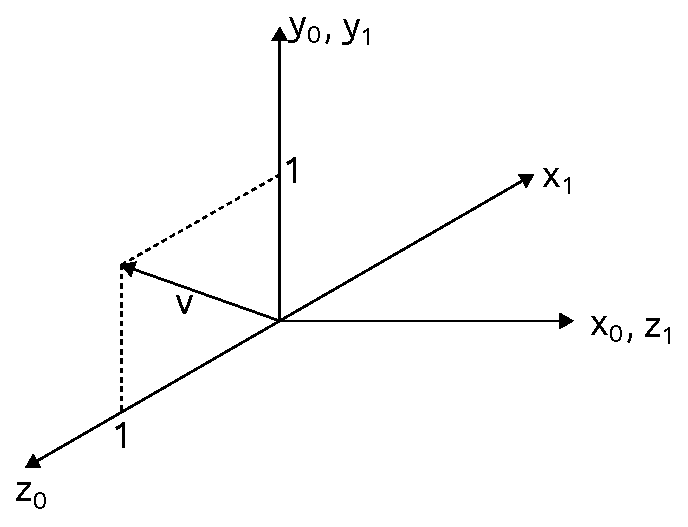
\includegraphics[width=0.5\textwidth]{figures/similarity_transform.eps}
        % \caption{\footnotesize }
    \end{figure}

\end{frame}

\begin{frame}
    \frametitle{Example 2.4 -- Revisited}

    Furthermore,
    \begin{align*}
      [B] = [P]^{-1}[A][P] &= \bmat{0 & 0 & -1 \\ 0 & 1 & 0 \\ 1 & 0 & 0}
      \bmat{c_\theta & -s_\theta & 0 \\ s_\theta & c_\theta & 0 \\ 0 & 0 & 1}
      \bmat{0 & 0 & 1 \\ 0 & 1 & 0 \\ -1 & 0 & 0} \\ &= 
      \bmat{1 & 0 & 0 \\ 0 & c_\theta & s_\theta \\ 0 & -s_\theta & c_\theta} = 
      R_{-x, \theta}.
    \end{align*}
\end{frame}

\end{document}
